\documentclass[10pt,letterpaper]{article}
\usepackage[utf8]{inputenc}
\usepackage[T1]{fontenc}
\usepackage{lmodern}
\usepackage[letterpaper,top=2.0cm,bottom=2.0cm,left=2.0cm,right=2.0cm]{geometry}
\usepackage{amsmath,amssymb}
\usepackage{booktabs}
\usepackage{tabularx}
\usepackage{xltabular}
\usepackage{pdflscape}
\usepackage{colortbl}
\usepackage{microtype}
\usepackage{array}
\usepackage{xcolor}
\usepackage{graphicx}
\graphicspath{{figuras/}{./}}
\usepackage{float}
\usepackage{fancyhdr}
\usepackage{tcolorbox}
\tcbuselibrary{skins,breakable}
\usepackage{hyperref}
\usepackage{titlesec}
\usepackage{enumitem}
\usepackage{lastpage}
\usepackage{caption}
\usepackage{pdfpages}

\renewcommand{\contentsname}{Índice General}
\renewcommand{\listtablename}{Índice de Cuadros}
\renewcommand{\listfigurename}{Índice de Figuras}
\captionsetup[table]{name=Cuadro,labelfont=bf,textfont=bf,skip=4pt}
\captionsetup[figure]{name=Figura,labelfont=bf,textfont=bf,skip=4pt}

\setlist{nosep,leftmargin=1.3em}
\setlength{\parindent}{0pt}
\setlength{\parskip}{3.5pt}

\definecolor{navyblue}{RGB}{26, 79, 124}
\definecolor{accentblue}{RGB}{51, 124, 207}
\definecolor{darkred}{RGB}{140, 30, 30}
\definecolor{forestgreen}{RGB}{20, 120, 40}
\definecolor{ambercolor}{RGB}{180, 100, 10}
\definecolor{boxbg}{RGB}{250, 251, 253}
\definecolor{tableheader}{RGB}{26, 79, 124}
\definecolor{tablerowalt}{RGB}{242, 247, 250}
\definecolor{grayborder}{RGB}{217, 217, 217}

\titleformat{\section}{\large\bfseries\color{navyblue}}{\thesection.}{0.5em}{}
\titleformat{\subsection}{\normalsize\bfseries\color{navyblue}}{\thesubsection.}{0.5em}{}
\titleformat{\subsubsection}{\small\bfseries\color{accentblue}}{\thesubsubsection.}{0.5em}{}
\titlespacing*{\section}{0pt}{5pt}{2pt}
\titlespacing*{\subsection}{0pt}{4pt}{1pt}
\titlespacing*{\subsubsection}{0pt}{3pt}{1pt}

\pagestyle{fancy}
\fancyhf{}
\lhead{\small\color{navyblue}\textbf{Solvanta Engineering Solutions} \textbar\ DPyPQ}
\rhead{\small PIB-01 \textbar\ Paquete de Ingeniería Básica}
\cfoot{\small Página \thepage\ de \pageref{LastPage}}
\renewcommand{\headrulewidth}{0.4pt}
\renewcommand{\footrulewidth}{0pt}
\setlength{\headheight}{14pt}

\hypersetup{
    colorlinks=true,
    linkcolor=navyblue,
    citecolor=navyblue,
    urlcolor=accentblue,
    pdfauthor={Solvanta Engineering Solutions S.A. de C.V.},
    pdftitle={PIB-01: Integración y Verificación del Paquete de Ingeniería Básica}
}

\begin{document}

% ==============================================================================
% PORTADA OFICIAL
% ==============================================================================
\begin{titlepage}
    \centering
    
\includegraphics[width=0.26\textwidth]{figuras/logo_empresa.png}\\[0.25cm]
    {\scshape\Large Benemérita Universidad Autónoma de Puebla}\\[0.1cm]
    {\scshape\large Facultad de Ingeniería Química \textbar\ Colegio de Ingeniería Química}\\[0.1cm]
    {\large Diseño de Procesos y Productos Químicos (DPyPQ)}\\[0.1cm]
    {\small Catedrático: Dr. Jesús Andrés Arzola Flores}\\[0.35cm]
    \hrule height 2pt
    \vspace{0.25cm}
    {\Huge \bfseries \color{navyblue} PIB-01\par}
    \vspace{0.15cm}
    {\LARGE \bfseries Integración y Verificación del\\[0.1cm] Paquete de Ingeniería Básica\par}
    \vspace{0.25cm}
    \hrule height 1pt
    \vspace{0.4cm}
    
    \begin{tcolorbox}[colframe=navyblue,colback=boxbg,arc=2mm,boxrule=0.8pt]
        \centering\small
        \setlength{\tabcolsep}{6pt}
        \renewcommand{\arraystretch}{1.2}
        \begin{tabularx}{\linewidth}{>{\bfseries\color{navyblue}}p{4.2cm} X}
            \toprule
            Proyecto & Planta de Producción de e-Metanol Grado Químico AA ($30\,000\text{ t/año}$) a partir de $\text{CO}_2$ Capturado e $\text{H}_2$ Verde Vía Electrólisis SOEC de Alta Temperatura \\
            Firma de ingeniería & Solvanta Engineering Solutions S.A. de C.V. \\
            Integrantes & Ing. Karol Paola Camacho López \textbar\ Ing. Paulina Mota Macip \newline
                          Ing. Gildardo Ocaña Barrales \textbar\ Ing. Grecia Figueroa Rincón \\
            Responsable del documento & Ing. Karol Paola Camacho López (Directora de Proyecto) \\
            Revisor técnico & Ing. Paulina Mota Macip (Especialista en Simulación e Instrumentación) \\
            Número de documento & \textbf{Solvanta-PIB-01} \\
            Revisión & \textbf{Rev. 0} (Emisión Oficial del Paquete de Ingeniería Básica) \\
            Fecha de emisión & 28 de Octubre de 2026 \\
            Código de licitación & \textbf{RFP-CCM-EM-001} \textbar\ Circular Carbon México, S.A. de C.V. \\
            \bottomrule
        \end{tabularx}
    \end{tcolorbox}
    
    \vspace{0.25cm}
    \begin{tcolorbox}[colframe=navyblue,colback=white,arc=2mm,boxrule=0.8pt]
        \centering
        \textbf{\color{navyblue}\normalsize Repositorio Oficial del Proyecto en GitHub}\\[2pt]
        \href{https://github.com/karolcamachol29-sudo/RFP-CCM-EM-001}{\texttt{\textbf{https://github.com/karolcamachol29-sudo/RFP-CCM-EM-001}}}\\[2pt]
        \footnotesize
        \textbf{Rama:} \texttt{main} \quad $\bullet$ \quad \textbf{Licitación:} \texttt{RFP-CCM-EM-001}\\[1pt]
        \textbf{Carpeta del Entregable:} \texttt{Entregables/PIB-01\_Solvanta/}\\
        \textbf{Documentos Vinculantes:} DWSIM v1, LE-01 Rev. 1, DTI v0.2, MCE-01 Rev. 1, AC-HAZOP-01
    \end{tcolorbox}
    
    \vfill
    {\footnotesize \textit{Expediente técnico integrador de ingeniería básica. Cumple estrictamente con la guía académica PIB-01 y las normas internacionales ANSI/ISA-5.1, ISO 10628, IEC 61882 y API RP 500.}\\
    Puebla, Pue. \textbar\ Ciclo Otoño 2026 \textbar\ Solvanta Engineering Solutions S.A. de C.V. \copyright\ Todos los derechos reservados.}
\end{titlepage}

% ==============================================================================
% CONTROL DE REVISIONES
% ==============================================================================
\section*{Control de Revisiones}
\addcontentsline{toc}{section}{Control de Revisiones}

\begin{table}[H]
\centering\small
\setlength{\tabcolsep}{6pt}
\renewcommand{\arraystretch}{1.2}
\begin{tabularx}{\textwidth}{c c X c c}
\toprule
\rowcolor{tableheader}
\color{white}\textbf{Revisión} & \color{white}\textbf{Fecha} & \color{white}\textbf{Descripción del Cambio} & \color{white}\textbf{Elaboró} & \color{white}\textbf{Revisó} \\
\midrule
0 & 28/10/2026 & Emisión inicial del Paquete de Ingeniería Básica (PIB-01), integrando Bases de Diseño consolidadas, Inventario Técnico de Equipos, Balance de Recursos y Servicios, Registro de Pendientes, Memoria Descriptiva, Arreglo General Preliminar y Resumen de Hallazgos HAZOP. & Equipo Solvanta & Dir. Técnica \\
1 & --- & Reservada para integración de resultados tecno-económicos BioSTEAM. & --- & --- \\
2 & --- & Reservada para actualización post-ingeniería de detalle. & --- & --- \\
\bottomrule
\end{tabularx}
\end{table}

\begin{tcolorbox}[colframe=ambercolor,colback=boxbg,arc=2mm,boxrule=1pt,title=\textbf{Advertencia Técnica Oficial}]
\small
La firma conservará permanentemente el historial de revisiones del expediente. No se sustituirá ningún documento previamente emitido sin registrar formalmente el número de modificación, la fecha de aprobación, el ingeniero responsable y el inventario exhaustivo de documentos técnicos afectados, preservando la trazabilidad documental hacia las fases subsecuentes del proyecto licitatorio.
\end{tcolorbox}

\vspace{0.3cm}
\tableofcontents
\vspace{0.3cm}
\listoftables
\vspace{0.3cm}
\listoffigures
\newpage

% ==============================================================================
% SECCIÓN 1: INTRODUCCIÓN Y MARCO CONCEPTUAL
% ==============================================================================
\section{Introducción y Marco Conceptual de la Actividad PIB-01}

\subsection{¿Qué es un Paquete de Ingeniería Básica?}
Un Paquete de Ingeniería Básica (PIB) es el compendio documental, técnico y analítico que sintetiza de forma integral la definición conceptual y de ingeniería de proceso para una planta industrial. Constituye el hito de cierre de la ingeniería conceptual y el insumo de entrada vinculante e inalterable para la ingeniería de detalle, la procura de equipos mayores y la evaluación económica y de riesgo.

El propósito central del presente expediente PIB-01 para la firma \textbf{Solvanta Engineering Solutions S.A. de C.V.} es reunir en un único cuerpo técnico:
\begin{itemize}
    \item La capacidad nominal de producción y regímenes máximos permisibles;
    \item Las condiciones termodinámicas e hidráulicas de operación en cada unidad física;
    \item El inventario técnico consolidado de equipos mecánicos, eléctricos y recipientes;
    \item El balance riguroso de materias primas, insumos, servicios auxiliares, consumibles y efluentes;
    \item El arreglo general preliminar (Plot Plan) con distancias seguras, rutas de escape y clasificación de áreas;
    \item La incorporación de las recomendaciones de seguridad derivadas del estudio HAZOP y la matriz causa--efecto; y
    \item El catálogo formal de datos pendientes (TBD) e inconsistencias controladas.
\end{itemize}

\begin{tcolorbox}[colframe=navyblue,colback=boxbg,arc=2mm,boxrule=1pt,title=\textbf{Criterio de Ingeniería y Coherencia Multidisciplinar}]
\small
El Paquete de Ingeniería Básica PIB-01 no es una colección inconexa de tablas numéricas. Todos y cada uno de los valores consignados en los formatos F-PIB-01, F-PIB-02, F-PIB-03 y F-PIB-04 corresponden rigurosamente al mismo modelo de proceso convergido en \texttt{DWSIM v10.2.4} (paquete \textbf{PRSV2-VL}), al Diagrama de Flujo de Proceso (\textbf{DFP v1}), a la Lista Maestra de Equipos (\textbf{LE-01 Rev. 1}), a la Filosofía de Control (\textbf{FC-01}), a la Matriz de Interbloqueos (\textbf{MI-01 / MCE-01 Rev. 1}) y al Expediente Técnico HAZOP (\textbf{AC-HAZOP-01}).
\end{tcolorbox}

\subsection{Ubicación dentro del Ciclo de Vida del Proyecto}
La secuencia metodológica del proyecto licitatorio \texttt{RFP-CCM-EM-001} se articula en la siguiente cadena documental:
\begin{center}
\small
\textbf{Bases de Diseño} $\longrightarrow$ \textbf{DWSIM v1} $\longrightarrow$ \textbf{PFD/DFP v1} $\longrightarrow$ \textbf{FC-01} $\longrightarrow$ \textbf{DTI v0.2} $\longrightarrow$ \textbf{HAZOP} $\longrightarrow$ \textbf{DTI v1.0} $\longrightarrow$ \textbf{PIB-01} $\longrightarrow$ \textbf{BioSTEAM / Evaluación Económica}
\end{center}

\subsection{Objetivo de la Actividad}
Integrar, estructurar y verificar la totalidad de la información técnica principal de la planta de producción de e-metanol ($30\,000\text{ t/año}$), recuperando las Bases de Diseño, la simulación DWSIM validada, los diagramas de ingeniería, los requerimientos de control y los hallazgos del taller HAZOP, conformando un expediente coherente que describa capacidades, equipos, recursos, servicios, efluentes y acciones pendientes del proyecto.

\subsection{Alcance Disciplinar: Inclusiones y Exclusiones Formales}
\textbf{PIB-01 incluye:}
\begin{itemize}
    \item Memoria descriptiva del proceso articulada en sus 17 puntos regulatorios;
    \item Formato F-PIB-01: Bases consolidadas de producción, límites de batería y supuestos;
    \item Formato F-PIB-02 (Partes A, B y C): Inventario técnico exhaustivo de los 30 equipos del proceso;
    \item Formato F-PIB-03 (Partes A y B): Balance de materias primas, servicios y salidas con cálculo anualizado;
    \item Plano de Arreglo General Preliminar (Solvanta\_AG-01) en plano independiente e integrado;
    \item Resumen técnico del tratamiento de los hallazgos HAZOP y salvaguardas de ingeniería;
    \item Formato F-PIB-04 (Partes A y B): Registro de pendientes técnicos (TBD), inconsistencias y acciones; y
    \item Acta de auditoría y verificación cruzada de la firma de ingeniería.
\end{itemize}

\textbf{PIB-01 no incluye:}
\begin{itemize}
    \item Estimaciones de costos de capital (CAPEX) o costos operativos (OPEX);
    \item Análisis económico financiero (VAN, TIR, tiempo de retorno o precio nivelado LCOMe);
    \item Dimensionamiento mecánico de detalle de tuberías (selección de Schedule, diámetros nominales o espesores de pared);
    \item Análisis de esfuerzos de flexibilidad por elementos finitos (CAESAR II); ni
    \item Cotizaciones comerciales formales de proveedores o selección definitiva de marcas.
\end{itemize}

\begin{tcolorbox}[colframe=darkred,colback=boxbg,arc=2mm,boxrule=1pt,title=\textbf{Advertencia Técnica Sobre Evaluación Económica}]
\small
En estricto cumplimiento de la guía docente, este expediente \textbf{no calcula costos ni indicadores económicos}. Su alcance se circunscribe a organizar y validar de manera indiscutible la información técnica de proceso que servirá de insumo para la fase posterior de modelado tecno-económico en la plataforma \textbf{BioSTEAM}.
\end{tcolorbox}

\subsection{Documentos de Entrada Oficiales Congelados}
Para la elaboración de este paquete se utilizó la última revisión aprobada de los siguientes documentos:
\begin{enumerate}
    \item \textbf{Bases de Diseño de Licitación RFP-CCM-EM-001 (Rev. 1):} Requerimientos de producto y sitio.
    \item \textbf{Simulación rigurosa DWSIM v10.2.4 (Archivo \texttt{Simulacion\_pruebas.dwxml}):} Paquete termodinámico PRSV2-VL convergido sin errores de entalpía o equilibrio.
    \item \textbf{Diagrama de Flujo de Proceso DFP v1.0 (\texttt{DFP-v1\_Solvanta.pdf}):} Plano oficial emitido en LE-01.
    \item \textbf{Tabla Oficial de Corrientes TC-01 Rev. 1 (\texttt{TC-01\_Solvanta.pdf}):} Balances de masa y composiciones.
    \item \textbf{Tabla Oficial de Energía y Servicios TE-01 Rev. 1 (\texttt{TE-01\_Solvanta.pdf}):} Consumos térmicos y eléctricos.
    \item \textbf{Lista Maestra de Equipos LE-01 Rev. 1 (\texttt{LE-01\_Solvanta.pdf}):} Catálogo de las 30 unidades físicas.
    \item \textbf{Diagrama de Tuberías e Instrumentación DTI v0.2 (\texttt{DTI-v0.2\_Solvanta.pdf}):} Base del estudio de riesgos.
    \item \textbf{Expediente Técnico HAZOP y MCE-01 Rev. 1 (\texttt{Solvanta\_AC-HAZOP-01\_Expediente.pdf}):} 42 desviaciones y 4 interlocks mayores.
    \item \textbf{Estudio Ambiental y Análisis de Ciclo de Vida AC-AMB-01 / E1.6:} Matriz de aspectos ambientales.
    \item \textbf{Hojas de Datos de Seguridad (HDS / FDS):} Metanol, Hidrógeno, Dióxido de Carbono y Oxígeno según SGA.
\end{enumerate}

\newpage
% ==============================================================================
% SECCIÓN 2: BASES CONSOLIDADAS DEL PROCESO (F-PIB-01)
% ==============================================================================
\section{F-PIB-01: Bases Consolidadas del Proceso}

\subsection{Propósito y Justificación de Parámetros}
El formato \textbf{F-PIB-01} consolida el conjunto de parámetros rectores sobre los cuales se dimensionó la planta de e-metanol. Responde de manera taxativa: ¿qué se produce?, ¿cuánto se produce?, ¿durante cuántas horas se opera?, ¿cuál es la calidad química exigida? y ¿cuáles son las fronteras de batería?

\subsection{Cálculos Matemáticos de Producción y Disponibilidad}
A continuación se presentan las operaciones matemáticas detalladas que fundamentan los valores del Cuadro \ref{tab:fpib01}:

\subsubsection{Cálculo de Disponibilidad Planeada}
Considerando un régimen continuo de operación petroquímica donde la planta funciona 24 horas al día durante 333.3 días al año, y reservando 31.7 días ($760\text{ h/año}$) para la parada programada anual por mantenimiento preventivo, inspección reglamentaria de recipientes a presión e inspección de celdas SOEC, se tiene:
\begin{equation}
\text{Horas efectivas anuales } (t_{\text{op}}) = 8\,000\,\frac{\text{h}}{\text{año}}
\end{equation}
\begin{equation}
\text{Horas totales del año calendario } (t_{\text{año}}) = 365\,\text{días} \times 24\,\frac{\text{h}}{\text{día}} = 8\,760\,\frac{\text{h}}{\text{año}}
\end{equation}
\begin{equation}
\text{Disponibilidad planeada } (\eta_{\text{disp}}) = \frac{t_{\text{op}}}{t_{\text{año}}} \times 100 = \frac{8\,000\,\text{h/año}}{8\,760\,\text{h/año}} \times 100 = \mathbf{91.32\%}
\end{equation}

\subsubsection{Cálculo de la Capacidad y Producción Anual Nominal}
A partir del flujo másico nominal de la corriente de e-metanol grado AA purificado a la salida del subenfriador \texttt{E-603} (\textbf{Corriente S-604} en la simulación \texttt{DWSIM v1}):
\begin{equation}
\dot{m}_{\text{MeOH, nominal}} = 3\,788.65\,\frac{\text{kg}}{\text{h}} \quad \left(118.341\,\frac{\text{kmol}}{\text{h}}\right)
\end{equation}
La masa anual producida bajo operación nominal ininterrumpida durante las 8,000 horas efectivas resulta:
\begin{equation}
\text{Producción anual}_{\text{nominal}} = \dot{m}_{\text{MeOH, nominal}} \times t_{\text{op}} = 3\,788.65\,\frac{\text{kg}}{\text{h}} \times 8\,000\,\frac{\text{h}}{\text{año}} = 30\,309\,200\,\frac{\text{kg}}{\text{año}}
\end{equation}
\begin{equation}
\text{Producción anual}_{\text{nominal}} = \frac{30\,309\,200\,\text{kg/año}}{1\,000\,\text{kg/t}} = \mathbf{30\,309.20\,\frac{\text{t}}{\text{año}}}
\end{equation}
Este valor de diseño cumple y supera con holgura técnica la meta contractual de la licitación Pemex ($30\,000\text{ t/año}$), absorbiendo pequeñas perturbaciones de pureza o arranques transitorios.

\subsubsection{Cálculo de la Capacidad Máxima de Diseño (+10\%)}
De acuerdo con las mejores prácticas de ingeniería de procesos (Towler \& Sinnott, 2021), los equipos dinámicos y columnas se verifican con un factor de sobre-diseño hidráulico del $10\%$ ($f_{\text{over}} = 1.10$):
\begin{equation}
\dot{m}_{\text{MeOH, máx}} = 1.10 \times \dot{m}_{\text{MeOH, nominal}} = 1.10 \times 3\,788.65\,\frac{\text{kg}}{\text{h}} = \mathbf{4\,167.52\,\frac{\text{kg}}{\text{h}}}
\end{equation}
\begin{equation}
\text{Producción anual}_{\text{máx}} = 4\,167.52\,\frac{\text{kg}}{\text{h}} \times 8\,000\,\frac{\text{h}}{\text{año}} \times \frac{1\,\text{t}}{1\,000\,\text{kg}} = \mathbf{33\,340.12\,\frac{\text{t}}{\text{año}}}
\end{equation}

\subsubsection{Cálculo de Consumo de Materias Primas Anuales}
Para el dióxido de carbono capturado (\textbf{Corriente S-101}) y el agua fresca make-up (\textbf{Corriente S-201}):
\begin{equation}
\dot{M}_{\text{CO}_2\text{, anual}} = 5\,274.34\,\frac{\text{kg}}{\text{h}} \times 8\,000\,\frac{\text{h}}{\text{año}} \times \frac{1\,\text{t}}{1\,000\,\text{kg}} = \mathbf{42\,194.72\,\frac{\text{t}}{\text{año}}}
\end{equation}
\begin{equation}
\dot{M}_{\text{Agua make-up, anual}} = 9\,241.84\,\frac{\text{kg}}{\text{h}} \times 8\,000\,\frac{\text{h}}{\text{año}} \times \frac{1\,\text{t}}{1\,000\,\text{kg}} = \mathbf{73\,934.72\,\frac{\text{t}}{\text{año}}} \quad (\approx 73\,934.72\,\text{m}^3\text{/año})
\end{equation}

\subsection{Formato F-PIB-01 Consolidado}
El Cuadro \ref{tab:fpib01} presenta el formato oficial F-PIB-01 con las 15 filas técnicas completas, erradicando los ejemplos didácticos de la plantilla.

\begin{landscape}
\footnotesize
\setlength{\tabcolsep}{4pt}
\begin{xltabular}{\linewidth}{|l|p{2.8cm}|p{3.5cm}|p{3.0cm}|c|p{3.2cm}|>{\raggedright\arraybackslash}X|c|}
\caption{\textbf{Formato F-PIB-01: Bases consolidadas del proceso.}} \label{tab:fpib01} \\ \hline
\rowcolor{tableheader}\color{white}\textbf{ID} & \color{white}\textbf{Parámetro} & \color{white}\textbf{Descripción} & \color{white}\textbf{Valor / Definición} & \color{white}\textbf{Unidad} & \color{white}\textbf{Fuente} & \color{white}\textbf{Supuesto / Método de Cálculo} & \color{white}\textbf{Estado} \\ \hline
\endfirsthead
\multicolumn{8}{c}{\footnotesize\textit{Continuación del Cuadro \ref{tab:fpib01} - Formato F-PIB-01}} \\ \hline
\rowcolor{tableheader}\color{white}\textbf{ID} & \color{white}\textbf{Parámetro} & \color{white}\textbf{Descripción} & \color{white}\textbf{Valor / Definición} & \color{white}\textbf{Unidad} & \color{white}\textbf{Fuente} & \color{white}\textbf{Supuesto / Método de Cálculo} & \color{white}\textbf{Estado} \\ \hline
\endhead
\hline \multicolumn{8}{r}{\footnotesize\textit{Continúa en la siguiente página...}} \\
\endfoot
\hline
\endlastfoot
BD-01 & Capacidad nominal & Producción horaria esperada de e-metanol durante operación normal habitual. & 3\,788.65 & kg/h & DWSIM v1; Corriente S-604; Licitación RFP-CCM-EM-001 & Operación continua al 100\% de carga en régimen estacionario (118.34 kmol/h de metanol puro). & Definido \\ \hline
BD-02 & Horas de operación & Horas efectivas acumuladas de régimen de producción durante un año. & 8\,000 & h/año & Bases de Diseño Rev. 1; LE-01K Supuesto 1 & Considera 333.3 días continuos a plena carga y 31.7 días (760 h) de paro anual para mantenimiento preventivo. & Definido \\ \hline
BD-03 & Producción anual & Masa total acumulada de e-metanol grado AA producida en las horas efectivas. & 30\,309.20 & t/año & Cálculo BD-03; DWSIM v1 & $= 3\,788.65\text{ kg/h} \times 8\,000\text{ h/año} / 1\,000$. Cumple y supera la meta contractual ($30\,000\text{ t/año}$). & Definido \\ \hline
BD-04 & Capacidad máxima & Mayor tasa permitida bajo condición de sobre-diseño hidráulico y térmico (+10\%). & 4\,167.52 & kg/h & Criterio de diseño de ingeniería de detalle (+10\%) & $= 1.10 \times 3\,788.65\text{ kg/h}$ ($33\,340.12\text{ t/año}$). Permite absorber picos de generación renovable o transitorios. & Definido \\ \hline
BD-05 & Disponibilidad planeada & Relación porcentual entre horas efectivas y horas del año calendario. & 91.32 & \% & Cálculo de disponibilidad operacional & $= (8\,000\text{ h} / 8\,760\text{ h}) \times 100$. Factor de servicio típico en complejos petroquímicos continuos de Pemex. & Definido \\ \hline
BD-06 & Producto principal & Compuesto químico sintetizado destinado a comercialización industrial. & e-Metanol Grado Químico AA & No aplica & Bases de Licitación RFP-CCM-EM-001; DWSIM v1 & Metanol sintético a partir de $\text{CO}_2$ capturado e $\text{H}_2$ verde vía electrólisis SOEC de vapor a alta temperatura. & Definido \\ \hline
BD-07 & Especificación del producto & Requisitos de calidad fisicoquímica comercial exigidos para metanol Grado AA. & Pureza $\ge 99.85\%$ p/p (obtenido $99.89\%$), $\text{H}_2\text{O} \le 0.10\%$ p/p, Densidad $0.791-0.793\text{ g/cm}^3$ & No aplica & Norma ASTM D1152; IMP / Pemex Petroquímica & Cumplimiento riguroso de pureza para uso como solvente y precursor químico (libre de etanol y acetona). & Definido \\ \hline
BD-08 & Materia prima principal & Insumos esenciales transformados estequiométricamente en el proceso. & $\text{CO}_2$ de captura externa ($\ge 99.0\%$ molar) y Agua desmineralizada para electrólisis & No aplica & Bases de Licitación; Conagua; LE-01 & $\text{CO}_2$ suministrado desde captura en polo industrial adyacente; agua provista de red industrial con $43.1\%$ de reciclo interno ZLD. & Definido \\ \hline
BD-09 & Modo de operación & Régimen temporal de marcha continua de la instalación industrial. & Continuo (24 horas/día, 7 días/semana) & No aplica & Filosofía de Operación FO-01; LE-01 & Operación continua en estado estacionario con control regulatorio avanzado y sistemas de paro SIS. & Definido \\ \hline
BD-10 & Límite de batería de entrada & Frontera física y condiciones de entrega de materias primas y servicios auxiliares. & $\text{CO}_2$ gas a $20.0\text{ bar}$ y $25.0^\circ\text{C}$; Agua desm. a $20.0\text{ bar}$ y $25^\circ\text{C}$; Electricidad a $115\text{ kV}$ & No aplica & DTI v0.2; LE-01B; Diagramas de Límite de Batería & Recepción isobárica de $\text{CO}_2$ a $20\text{ bar}$ acoplado al $\text{H}_2$ SOEC, eliminando compresión in situ de $\text{CO}_2$. & Definido \\ \hline
BD-11 & Límite de batería de salida & Frontera física y condiciones de despacho de productos, subproductos y efluentes. & Metanol a TK-601 ($35^\circ\text{C}$, $1.013\text{ bar}$); $\text{O}_2$ puro a batería ($19.4\text{ bar}$, $31^\circ\text{C}$); Purga ($1.1\text{ bar}$) & No aplica & DTI v0.2; AC-HAZOP-01; TC-01 & Despacho a autotanques; venta de $\text{O}_2$ medicinal/industrial; gas de purga a red de gas combustible Pemex. & Definido \\ \hline
BD-12 & Condición ambiental referencia & Variables meteorológicas del emplazamiento en sitio industrial de referencia. & $T_{\text{amb}} = 25.0^\circ\text{C}$ media ($15-38^\circ\text{C}$), $P_{\text{amb}} = 1.013\text{ bar}$ (nivel del mar), Humedad $78\%$, Viento NNE & No aplica & Estación Meteorológica polo industrial adyacente; Conagua & Condiciones base para diseño térmico de intercambiadores, torres de enfriamiento y clasificación de áreas. & Definido \\ \hline
BD-13 & Caso normal de operación & Régimen de diseño representativo de la operación habitual balanceada. & Carga 100\%: $3\,788.65\text{ kg/h}$ MeOH, $5\,274.34\text{ kg/h}$ $\text{CO}_2$, $55\,436.39\text{ kW}$ potencia neta & No aplica & DWSIM v1 oficial; Balances TC-01 y TE-01 & Balance de materia y energía totalmente cerrado y validado termodinámicamente en DWSIM (Escenario D Óptimo). & Definido \\ \hline
BD-14 & Caso máximo de operación & Régimen operacional continuo límite permisible (+10\% sobre capacidad). & Carga 110\%: $4\,167.52\text{ kg/h}$ MeOH, $5\,801.77\text{ kg/h}$ $\text{CO}_2$, $60\,980.03\text{ kW}$ potencia neta & No aplica & Factor de diseño hidráulico y térmico de ingeniería & Permite evaluar la capacidad de bombeo, compresores y válvulas de control bajo transitorios controlados. & Definido \\ \hline
BD-15 & Módulo estequiométrico $M$ & Parámetro de alimentación al bucle: $M = (y_{\text{H}_2} - y_{\text{CO}_2})/(y_{\text{CO}} + y_{\text{CO}_2})$. & $2.05$ (Intervalo admisible: $2.00 - 2.10$) & Adimensional & Cinética Lurgi; Haldor Topsoe; DWSIM v1 & Exceso leve de hidrógeno ($M > 2.0$) que evita la coquización catalítica y maximiza selectividad a metanol. & Definido \\ \hline
\end{xltabular}
\end{landscape}

\newpage
% ==============================================================================
% SECCIÓN 3: INVENTARIO TÉCNICO DE EQUIPOS (F-PIB-02)
% ==============================================================================
\section{F-PIB-02: Inventario Técnico de Equipos}

\subsection{Propósito y Clasificación de Variables de Tamaño}
El formato \textbf{F-PIB-02} consolida el censo integral de las 30 unidades físicas del proceso, clasificadas en tres partes complementarias:
\begin{itemize}
    \item \textbf{Parte A (Cuadro \ref{tab:fpib02a}):} Identificación, servicio del equipo, cantidad de unidades (operación/reserva), capacidad normal y máxima, presión de operación y temperatura de operación.
    \item \textbf{Parte B (Cuadro \ref{tab:fpib02b}):} Variable representativa de tamaño, valor y unidad de tamaño, potencia mecánica/eléctrica consumida o carga térmica transferida (distinguiendo rigurosamente entre potencia y carga térmica), metalurgia preliminar y servicio auxiliar requerido.
    \item \textbf{Parte C (Cuadro \ref{tab:fpib02c}):} Requisitos derivados del análisis de riesgos HAZOP y filosofía de control, fuente documental, pendiente técnico específico y estado del dato.
\end{itemize}

\subsection{Distinción entre Potencia Mecánica/Eléctrica y Carga Térmica}
A fin de evitar penalizaciones técnicas, el expediente distingue formalmente:
\begin{enumerate}
    \item \textbf{Potencia ($W$, en kW):} Energía mecánica o eléctrica suministrada por unidad de tiempo a máquinas dinámicas como bombas centrífugas (\texttt{P-201}, \texttt{P-601}, \texttt{P-602}, \texttt{P-801}), turbocompresores (\texttt{C-301}), sopladores (\texttt{C-501}), el stack electrolítico (\texttt{EL-201}) o la energía recuperada en el turboexpansor (\texttt{EXP-501}).
    \item \textbf{Carga Térmica ($Q$, en kW):} Calor transferido por conducción/convección por unidad de tiempo a través de superficies de intercambio en enfriadores (\texttt{E-201}, \texttt{E-203}, \texttt{E-501}, \texttt{E-601}, \texttt{E-603}), calentadores/rehervidores (\texttt{E-301}, \texttt{E-602}), sobrecalentadores (\texttt{E-202}), intercambiadores de integración térmica (\texttt{E-502A/B}) o el calor exotérmico generado por la reacción en la caldera (\texttt{R-401-S}).
\end{enumerate}

\subsection{Formato F-PIB-02, Parte A: Identificación y Condiciones de Operación}
A continuación, el Cuadro \ref{tab:fpib02a} detalla la Parte A para la totalidad de equipos de la planta.

\begin{landscape}
\footnotesize
\setlength{\tabcolsep}{3.5pt}
\begin{xltabular}{\linewidth}{|l|p{2.6cm}|p{5.5cm}|c|r|r|r|r|}
\caption{\textbf{Formato F-PIB-02, Parte A: Identificación, capacidad y condiciones de operación.}} \label{tab:fpib02a} \\ \hline
\rowcolor{tableheader}\color{white}\textbf{Tag} & \color{white}\textbf{Tipo de Equipo} & \color{white}\textbf{Servicio del Equipo} & \color{white}\textbf{Cantidad} & \color{white}\textbf{Cap. Normal} & \color{white}\textbf{Cap. Máxima} & \color{white}\textbf{Presión Op.} & \color{white}\textbf{Temp. Op.} \\ \hline
\endfirsthead
\multicolumn{8}{c}{\footnotesize\textit{Continuación del Cuadro \ref{tab:fpib02a} - F-PIB-02, Parte A}} \\ \hline
\rowcolor{tableheader}\color{white}\textbf{Tag} & \color{white}\textbf{Tipo de Equipo} & \color{white}\textbf{Servicio del Equipo} & \color{white}\textbf{Cantidad} & \color{white}\textbf{Cap. Normal} & \color{white}\textbf{Cap. Máxima} & \color{white}\textbf{Presión Op.} & \color{white}\textbf{Temp. Op.} \\ \hline
\endhead
\hline \multicolumn{8}{r}{\footnotesize\textit{Continúa en la siguiente página...}} \\
\endfoot
\hline
\endlastfoot
P-201A/B & Bomba centrífuga & Impulso de agua desmineralizada make-up hacia caldera de chaqueta R-401-S & 2: 1 op / 1 res & 9\,241.8 kg/h & 10\,166.0 kg/h & 20.00 bar & 25.0 $^\circ$C \\ \hline
MIX-201 & Mezclador estático & Mezcla homogénea de agua fresca make-up y retorno condensado ZLD & 1 unidad & 16\,244.9 kg/h & 17\,869.4 kg/h & 20.00 bar & 39.8 $^\circ$C \\ \hline
R-401-S & Caldera acoplada reactor & Generación de vapor saturado a 20 bar absorbiendo calor exotérmico de síntesis & 1 unidad & 16\,244.9 kg/h & 17\,869.4 kg/h & 20.00 bar & 212.4 $^\circ$C \\ \hline
E-202 & Sobrecalentador vapor & Sobrecalentamiento eléctrico de vapor saturado de 212.4 $^\circ$C a 800 $^\circ$C a SOEC & 1 unidad & 16\,244.9 kg/h & 17\,869.4 kg/h & 20.00 bar & 800.0 $^\circ$C \\ \hline
EL-201 & Electrolizador SOEC & Disociación catalítica de vapor a 800 $^\circ$C produciendo H2 verde y O2 & 1 módulo multi & 16\,244.9 kg/h & 17\,869.4 kg/h & 19.40 bar & 800.0 $^\circ$C \\ \hline
E-201 & Enfriador de O2 puro & Enfriamiento de oxígeno puro anódico de 800 $^\circ$C a 31 $^\circ$C con agua de torre & 1 unidad & 10\,098.8 kg/h & 11\,108.6 kg/h & 19.40 bar & 31.0 $^\circ$C \\ \hline
E-203 & Condensador efluente SOEC & Enfriamiento de gas catódico H2 húmedo de 800 $^\circ$C a 38 $^\circ$C para condensar H2O & 1 unidad & 6\,145.8 kg/h & 6\,760.4 kg/h & 19.40 bar & 38.0 $^\circ$C \\ \hline
V-201 & Separador flash KO Drum & Separación bifásica a 19.4 bar de hidrógeno verde seco y condensado hídrico & 1 recipiente vert. & 6\,145.8 kg/h & 6\,760.4 kg/h & 19.40 bar & 38.0 $^\circ$C \\ \hline
MIX-301 & Mezclador estático syngas & Unión de H2 verde seco y CO2 de captura para fijar módulo M = 2.05 & 1 unidad & 6\,589.1 kg/h & 7\,248.0 kg/h & 19.40 bar & 32.9 $^\circ$C \\ \hline
E-301 & Precalentador de syngas & Acondicionamiento térmico de gas fresco de 32.9 $^\circ$C a 71.7 $^\circ$C previo a C-301 & 1 unidad & 6\,589.1 kg/h & 7\,248.0 kg/h & 19.40 bar & 71.7 $^\circ$C \\ \hline
C-301 & Compresor centrífugo & Presurización multietapa de syngas fresco de 19.4 bar a 75.0 bar de síntesis & 1 tren multietapa & 6\,589.1 kg/h & 7\,248.0 kg/h & 75.00 bar & 271.0 $^\circ$C \\ \hline
MIX-401 & Mezclador bucle síntesis & Mezcla adiabática de syngas fresco comprimido con gas de reciclo circulante & 1 unidad & 21\,308.1 kg/h & 23\,438.9 kg/h & 75.00 bar & 83.2 $^\circ$C \\ \hline
E-502A/B & Economizador FEHE & Precalentamiento de mezcla reactiva a 210 $^\circ$C recuperando calor del efluente & 2 carcasas serie & 21\,308.1 kg/h & 23\,438.9 kg/h & 75.00 bar & 210.0 $^\circ$C \\ \hline
R-401 & Reactor tubular BWR Lurgi & Síntesis catalítica exotérmica de metanol sobre lecho Cu/ZnO/Al2O3 a 75 bar & 1 reactor multitub. & 21\,308.1 kg/h & 23\,438.9 kg/h & 75.00 bar & 245.0 $^\circ$C \\ \hline
E-501 & Condensador síntesis & Enfriamiento y condensación total de metanol/agua de 224.6 $^\circ$C a 38 $^\circ$C con CW & 1 unidad C\&T & 21\,308.1 kg/h & 23\,438.9 kg/h & 75.00 bar & 38.0 $^\circ$C \\ \hline
V-501 & Separador flash HP & Separación bifásica a 75 bar de metanol crudo líquido y gas inconvertido & 1 recipiente vert. & 21\,308.1 kg/h & 23\,438.9 kg/h & 75.00 bar & 38.0 $^\circ$C \\ \hline
SPLIT-501 & Divisor de reciclo/purga & Desvío de 96\% de gas inconvertido a reciclo y 4\% a purga continua de inertes & 1 cabezal control & 15\,339.8 kg/h & 16\,873.7 kg/h & 75.00 bar & 38.0 $^\circ$C \\ \hline
C-501 & Soplador de reciclo & Circulación forzada de gas de reciclo venciendo delta P = 1.5 bar del bucle & 1 soplador centríf. & 14\,726.2 kg/h & 16\,198.8 kg/h & 75.00 bar & 60.0 $^\circ$C \\ \hline
EXP-501 & Turboexpansor de purga & Despresurización criogénica de purga (75 a 1.1 bar) con recuperación eléctrica & 1 turboexpansor & 613.6 kg/h & 675.0 kg/h & 1.10 bar & -138.6 $^\circ$C \\ \hline
VALV-601 & Válvula expansión JT & Reducción isentálpica de presión de metanol crudo líquido de 75.0 a 1.25 bar & 1 válvula control & 5\,968.4 kg/h & 6\,565.2 kg/h & 1.25 bar & 38.0 $^\circ$C \\ \hline
V-601 & Flash desgasificador LP & Desorción de gases disueltos (CO2, H2, CH4) previo al fraccionamiento & 1 tambor horiz. & 5\,968.4 kg/h & 6\,565.2 kg/h & 1.25 bar & 38.0 $^\circ$C \\ \hline
P-601A/B & Bombas alim. destilación & Impulso de metanol crudo desgasificado de 1.25 a 2.20 bar a plato 18 de T-601 & 2: 1 op / 1 res & 5\,961.8 kg/h & 6\,558.0 kg/h & 2.20 bar & 38.0 $^\circ$C \\ \hline
T-601 & Columna fraccionadora & Destilación fraccionada para purificar e-metanol a Grado AA ($>99.85\%$ p/p) & 1 columna platos & 5\,961.8 kg/h & 6\,558.0 kg/h & 1.20 bar & 68.5 $^\circ$C \\ \hline
E-601 & Condensador domo T-601 & Condensación total de vapores de metanol en cabeza de columna (R/D = 1.50) & 1 intercambiador & 9\,471.6 kg/h & 10\,418.8 kg/h & 1.20 bar & 68.5 $^\circ$C \\ \hline
V-602 & Acumulador de reflujo & Acumulación y desacoplamiento de metanol destilado para reflujo y producto & 1 tambor horiz. & 9\,471.6 kg/h & 10\,418.8 kg/h & 1.20 bar & 68.5 $^\circ$C \\ \hline
P-602A/B & Bombas de reflujo y envío & Retorno de reflujo (5\,683 kg/h) y envío de metanol producto (3\,789 kg/h) & 2: 1 op / 1 res & 9\,471.6 kg/h & 10\,418.8 kg/h & 2.50 bar & 68.5 $^\circ$C \\ \hline
E-602 & Rehervidor de fondos T-601 & Suministro de vapor de despojo hídrico en fondo de torre con vapor de 3.5 bar & 1 termosifón vert. & 4\,346.8 kg/h & 4\,781.5 kg/h & 1.25 bar & 103.9 $^\circ$C \\ \hline
E-603 & Subenfriador de producto & Enfriamiento final de metanol Grado AA de 68.5 $^\circ$C a 35.0 $^\circ$C previo a almacenaje & 1 intercambiador & 3\,788.7 kg/h & 4\,167.5 kg/h & 1.10 bar & 35.0 $^\circ$C \\ \hline
TK-601 & Tanque almacenamiento MeOH & Almacenamiento atmosférico seguro con colchón de N2 (15 días de inventario) & 1 tanque vert. & 3\,788.7 kg/h & Despacho lote & 1.013 bar & 35.0 $^\circ$C \\ \hline
V-801 & Desaireador acumulador ZLD & Recepción y desgasificación de condensado SOEC y fondos hídricos de torre & 1 tambor vert. & 7\,004.4 kg/h & 7\,704.9 kg/h & 1.25 bar & 58.9 $^\circ$C \\ \hline
P-801A/B & Bombas retorno agua ZLD & Presurización de agua tratada desmineralizada de 1.25 a 20.0 bar a caldera & 2: 1 op / 1 res & 7\,004.4 kg/h & 7\,704.9 kg/h & 20.00 bar & 59.2 $^\circ$C \\ \hline
\end{xltabular}
\end{landscape}

\newpage
% ==============================================================================
% SECCIÓN 4: INVENTARIO TÉCNICO - PARTE B (TAMAÑO Y REQUERIMIENTOS)
% ==============================================================================
\subsection{Formato F-PIB-02, Parte B: Variables de Tamaño y Requerimientos}
El Cuadro \ref{tab:fpib02b} consigna la variable de tamaño representativa según la tipología física de cada equipo, el valor numérico con sus unidades, la distinción rigurosa de potencia vs carga térmica, los materiales de construcción preliminares y los servicios auxiliares requeridos.

\begin{landscape}
\footnotesize
\setlength{\tabcolsep}{3.5pt}
\begin{xltabular}{\linewidth}{|l|p{3.8cm}|p{3.2cm}|p{3.2cm}|p{3.8cm}|>{\raggedright\arraybackslash}X|}
\caption{\textbf{Formato F-PIB-02, Parte B: Variables de tamaño, potencia / carga térmica y servicios.}} \label{tab:fpib02b} \\ \hline
\rowcolor{tableheader}\color{white}\textbf{Tag} & \color{white}\textbf{Variable de Tamaño} & \color{white}\textbf{Valor / Unidad Tamaño} & \color{white}\textbf{Potencia / Carga Térmica} & \color{white}\textbf{Material Preliminar} & \color{white}\textbf{Servicio Auxiliar Requerido} \\ \hline
\endfirsthead
\multicolumn{6}{c}{\footnotesize\textit{Continuación del Cuadro \ref{tab:fpib02b} - F-PIB-02, Parte B}} \\ \hline
\rowcolor{tableheader}\color{white}\textbf{Tag} & \color{white}\textbf{Variable de Tamaño} & \color{white}\textbf{Valor / Unidad Tamaño} & \color{white}\textbf{Potencia / Carga Térmica} & \color{white}\textbf{Material Preliminar} & \color{white}\textbf{Servicio Auxiliar Requerido} \\ \hline
\endhead
\hline \multicolumn{6}{r}{\footnotesize\textit{Continúa en la siguiente página...}} \\
\endfoot
\hline
\endlastfoot
P-201A/B & Flujo volumétrico y carga hidráulica & 9.27 m³/h \textbar\ 195 m carga & Potencia: +6.42 kW eléctrico & Acero inoxidable 316L & Electricidad 440 V trifásica \\ \hline
MIX-201 & Flujo másico total procesado & 16.24 t/h mezcla líquida & No aplica (mezcla adiabática) & Acero inoxidable 316L & Ninguno (equipo estático pasivo) \\ \hline
R-401-S & Flujo de vapor y carga generada & 16.24 t/h vapor a 20 bar & Carga: -12\,335.36 kW térmicos & Acero al carbono A-516 Gr 70 & Agua tratada de caldera a 20 bar \\ \hline
E-202 & Potencia eléctrica sobrecalentamiento & 5\,248.42 kW térmicos & Pot. eléc. / Carga: +5\,248.42 kW & Inconel 625 / Alloy 800H & Electricidad media tensión / SCR \\ \hline
EL-201 & Potencia eléctrica y producción H2 & 38.07 MWe (Escenario D: 32.92 kWh/kg H2) \textbar\ 1\,314.8 kg/h H2 & Potencia: +38\,067.30 kW eléc. AC (36\,735.0 kW DC) & Celdas cerámicas YSZ/Ni-YSZ & Electricidad DC / Vapor a 800 $^\circ$C \\ \hline
E-201 & Área de transferencia de calor & 185.0 m² preliminar & Carga: -2\,345.10 kW térmicos & Acero inoxidable 316L & Agua de enfriamiento de torre (CW) \\ \hline
E-203 & Área de transferencia de calor & 340.0 m² preliminar & Carga: -8\,962.22 kW térmicos & Acero inoxidable 316L / Inconel & Agua de enfriamiento de torre (CW) \\ \hline
V-201 & Volumen útil y tiempo retención & 8.5 m³ (D=1.4 m, H=4.2 m) & No aplica (separación flash) & Acero inoxidable 316L & Aire de instrumentos para control LCV \\ \hline
MIX-301 & Flujo de gas syngas procesado & 6.59 t/h syngas combinado & No aplica (mezcla adiabática) & Acero inoxidable 316L & Ninguno (mezclador estático pasivo) \\ \hline
E-301 & Área de transferencia de calor & 42.0 m² preliminar & Carga: +250.00 kW térmicos & Acero al carbono A-516 Gr 70 & Vapor de baja presión (LP steam) \\ \hline
C-301 & Caudal de gas y relación compresión & 1\,850 Nm³/h \textbar\ Rc = 3.87 & Potencia: +1\,316.67 kW eléctrico & Acero forjado aleado Cr-Mo & Electricidad 4.16 kV / CW en aceite \\ \hline
MIX-401 & Flujo másico total bucle síntesis & 21.31 t/h combinadas & No aplica (mezcla adiabática) & Acero al carbono A-516 Gr 70 & Ninguno (equipo estático pasivo) \\ \hline
E-502A/B & Área de intercambio combinada & 165.0 m² serie (A/B) & Carga: 1\,235.43 kW intercambio & Acero aleado 1.25Cr-0.5Mo & Integración térmica interna de proceso \\ \hline
R-401 & Masa catalizador y número tubos & 18.5 t catalizador \textbar\ 2\,800 tubos & Carga: -7\,924.76 kW térmicos & Tubos: Aleado / Carcasa: CS & Generación de vapor en R-401-S \\ \hline
E-501 & Área de condensación bucle & 520.0 m² preliminar & Carga: -13\,742.75 kW térmicos & Acero al carbono A-516 / SS 316 & Agua de enfriamiento de torre (CW) \\ \hline
V-501 & Volumen útil de retención flash & 14.5 m³ (D=1.8 m, H=5.8 m) & No aplica (separación bifásica) & Acero al carbono Clad 316L & Aire de instrumentos para LCV y SDV \\ \hline
SPLIT-501 & Fracción de purga de inertes & 96.0\% reciclo \textbar\ 4.0\% purga & No aplica (divisor de flujo) & Acero al carbono A-516 Gr 70 & Aire de instrumentos para FCV-505 \\ \hline
C-501 & Caudal circulante y delta P bucle & 4\,120 m³/h \textbar\ delta P = 1.5 bar & Potencia: +150.00 kW eléctrico & Acero forjado aleado & Electricidad 440 V trifásica \\ \hline
EXP-501 & Potencia eléctrica recuperada & Generador acoplado 437.8 kW & Potencia: -437.79 kW generado & Acero aleado criogénico 304L & Exportación eléctrica a red interna \\ \hline
VALV-601 & Coeficiente de flujo requerido & $\text{Cv} = 14.5\text{ gpm/psi}^{0.5}$ & No aplica (laminación JT) & Cuerpo acero inoxidable 316L & Aire de instrumentos para LCV-501 \\ \hline
V-601 & Volumen útil desgasificación flash & 6.2 m³ (D=1.2 m, L=5.5 m) & No aplica (desorción física) & Acero al carbono A-516 Gr 70 & Aire de instrumentos / Venteo seguro \\ \hline
P-601A/B & Flujo volumétrico y carga hidráulica & 7.55 m³/h \textbar\ 22 m carga & Potencia: +1.20 kW eléctrico & Acero inoxidable 316L & Electricidad 440 V / Sellos mecánicos \\ \hline
T-601 & Número platos y diámetro torre & 34 platos mecánicos \textbar\ D=1.2 m & No aplica (separación fraccionada) & Carcasa e internos: SS 316L & Vapor en fondo y CW en condensador \\ \hline
E-601 & Área de transferencia de calor & 145.0 m² preliminar & Carga: -3\,077.25 kW térmicos & Acero inoxidable 316L & Agua de enfriamiento de torre (CW) \\ \hline
V-602 & Volumen de acumulación reflujo & 5.8 m³ (10 min retención) & No aplica & Acero inoxidable 316L & Aire de instrumentos para control LIC \\ \hline
P-602A/B & Flujo volumétrico y carga hidráulica & 12.0 m³/h \textbar\ 28 m carga & Potencia: +1.50 kW eléctrico & Acero inoxidable 316L & Electricidad 440 V prueba explosión \\ \hline
E-602 & Área de ebullición termosifón & 130.0 m² preliminar & Carga: +3\,266.68 kW térmicos & Tubos y carcasa: SS 316L & Vapor saturado de baja presión (3.5 bar) \\ \hline
E-603 & Área de subenfriamiento producto & 18.5 m² preliminar & Carga: -111.11 kW térmicos & Acero inoxidable 316L & Agua helada / Chilled water (7 $^\circ$C) \\ \hline
TK-601 & Capacidad nominal de inventario & 2\,000 m³ (D=14 m, H=13.5 m) & No aplica (almacenamiento estático) & Acero al carbono epóxico & Colchón permanente N2 / Red SCI \\ \hline
V-801 & Volumen de retención y desacople & 12.0 m³ (retención 1.5 h) & No aplica & Acero inoxidable 304L & Vapor de purga desaireación \\ \hline
P-801A/B & Flujo volumétrico y carga hidráulica & 7.10 m³/h \textbar\ 195 m carga & Potencia: +5.51 kW eléctrico & Acero inoxidable 316L & Electricidad 440 V trifásica \\ \hline
\end{xltabular}
\end{landscape}

\newpage
% ==============================================================================
% SECCIÓN 5: INVENTARIO TÉCNICO - PARTE C (TRAZABILIDAD Y REQUISITOS HAZOP)
% ==============================================================================
\subsection{Formato F-PIB-02, Parte C: Trazabilidad, Requisitos HAZOP y Pendientes}
El Cuadro \ref{tab:fpib02c} vincula cada unidad con las salvaguardas y modificaciones derivadas del análisis de riesgos HAZOP (\texttt{Solvanta\_AC-HAZOP-01}), la filosofía de control (\texttt{FC-01}), las fuentes documentales y el estado técnico específico.

\begin{landscape}
\footnotesize
\setlength{\tabcolsep}{3.5pt}
\begin{xltabular}{\linewidth}{|l|p{6.0cm}|p{3.2cm}|p{4.2cm}|c|}
\caption{\textbf{Formato F-PIB-02, Parte C: Requisitos HAZOP / control, fuentes y pendientes técnicos.}} \label{tab:fpib02c} \\ \hline
\rowcolor{tableheader}\color{white}\textbf{Tag} & \color{white}\textbf{Requisito HAZOP / Filosofía de Control} & \color{white}\textbf{Fuente Documental} & \color{white}\textbf{Pendiente Técnico Específico} & \color{white}\textbf{Estado} \\ \hline
\endfirsthead
\multicolumn{5}{c}{\footnotesize\textit{Continuación del Cuadro \ref{tab:fpib02c} - F-PIB-02, Parte C}} \\ \hline
\rowcolor{tableheader}\color{white}\textbf{Tag} & \color{white}\textbf{Requisito HAZOP / Filosofía de Control} & \color{white}\textbf{Fuente Documental} & \color{white}\textbf{Pendiente Técnico Específico} & \color{white}\textbf{Estado} \\ \hline
\endhead
\hline \multicolumn{5}{r}{\footnotesize\textit{Continúa en la siguiente página...}} \\
\endfoot
\hline
\endlastfoot
P-201A/B & Alarma PAL-201 por baja presión de descarga; conmutación automática a P-201B y válvula check de retención. & DWSIM v1; LE-01D; DTI v0.2 & Confirmar curva de bomba y NPSH disponible con catálogo de fabricante. & Preliminar \\ \hline
MIX-201 & Válvulas check antirretorno en líneas S-201 y S-202 para impedir contaminación o retorno de condensado ZLD. & DWSIM v1; DTI v0.2; FC-01 & Calcular caída de presión hidráulica definitiva (Delta P). & Definido \\ \hline
R-401-S & Válvula de alivio mecánico PSV-401 tarada a 24 bar con venteo a atmósfera segura; interlock I-01 por TAHH-401. & DWSIM v1; TE-01; AC-HAZOP-01 & Verificar espesor de chapa de caldera según código ASME Sección VIII Div. 1. & Definido \\ \hline
E-202 & TAH-202 de advertencia y termostato TAHH-202 ($>780^\circ\text{C}$) con corte directo a tiristores SCR de resistencias. & DWSIM v1; TE-01; DTI v0.2 & Diseñar lazo de control SCR y contactores principales de potencia. & Preliminar \\ \hline
EL-201 & Interlock I-03 por alta presión diferencial trans-membrana PDAHH-201 ($>0.40\text{ bar}$) con desenergización DC inmediata. & DWSIM v1; LE-01E; AC-HAZOP-01 & Incorporar curvas de degradación de celdas a 10 años en BioSTEAM (TBD-01). & TBD abierto \\ \hline
E-201 & Válvula de control de agua TCV-201 en posición Falla Abierta (Fail-Open) y válvula check en retorno de CW. & DWSIM v1; TE-01; DTI v0.2 & Obtener coeficiente global U riguroso mediante simulación en HTRI (TBD-02). & TBD abierto \\ \hline
E-203 & TAH-203 por alta temperatura en H2 de salida; válvula check en retorno de agua de enfriamiento. & DWSIM v1; TE-01; AC-HAZOP-01 & Determinar área TEMA y pérdida de carga con software HTRI (TBD-02). & TBD abierto \\ \hline
V-201 & Alarmas simples LAH-201 / LAL-201 con lazo regulatorio LCV-201 hacia circuito de agua condensada. & DWSIM v1; DTI v0.2; FC-01 & Verificar tiempo de retención de líquido (5 min a flujo nominal). & Definido \\ \hline
MIX-301 & Analizador en línea AIC-301 con lazo de control estequiométrico en alimentación de CO2 para fijar M=2.05. & DWSIM v1; LE-01C; FC-01 & Validar pérdida de carga interna en mezclador estático. & Definido \\ \hline
E-301 & TAH-301 para evitar sobrecalentamiento de syngas a succión de C-301; trampa de vapor en retorno. & DWSIM v1; TE-01; DTI v0.2 & Dimensionamiento de área de intercambio con vapor LP. & Preliminar \\ \hline
C-301 & Interlock I-02 por alta presión PSHH-301 con disparo de motor y apertura de lazo anti-surge UIC-301. & DWSIM v1; TE-01; AC-HAZOP-01 & Solicitar curva de compresión y especificación anti-surge a fabricante (TBD-03). & TBD abierto \\ \hline
MIX-401 & Válvulas check en descargas de C-301 y C-501 impidiendo flujo inverso entre bucle y gas fresco. & DWSIM v1; LE-01C; DTI v0.2 & Calcular caída de presión del cabezal mezclador. & Definido \\ \hline
E-502A/B & Válvula de control bypass TV-502 para modular temperatura de entrada a reactor a 210 $^\circ$C según TIC-401. & DWSIM v1; LE-01E; DTI v0.2 & Calcular área rigurosa y coeficiente U en ambas carcasas en HTRI (TBD-02). & TBD abierto \\ \hline
R-401 & Interlock I-01 por embalamiento térmico TAHH-401 ($>260^\circ\text{C}$) con cierre inmediato de SDV-301 y desvío a reciclo. & DWSIM v1; LE-01C; AC-HAZOP-01 & Ajustar cinética de desactivación catalítica a lo largo de 4 años (TBD-01). & TBD abierto \\ \hline
E-501 & TAH-501 por alta temperatura de salida ($>42^\circ\text{C}$); válvula de agua TCV-501 en Falla Abierta (FO). & DWSIM v1; TE-01; AC-HAZOP-01 & Dimensionamiento TEMA con agua de enfriamiento en HTRI (TBD-02). & TBD abierto \\ \hline
V-501 & Interlock I-04 por muy bajo nivel LALL-501 con cierre estanco de SDV-501 (anti gas blow-by) hacia V-601. & DWSIM v1; AC-HAZOP-01; DTI v0.2 & Especificar actuador neumático de SDV-501 con cierre menor a 1.0 s (HZ-02). & En revisión \\ \hline
SPLIT-501 & Lazo de control de flujo FIC-505 en purga continua manteniendo concentración de inertes $<3.5\%$ molar. & DWSIM v1; LE-01E; DTI v0.2 & Confirmar porcentaje de purga mediante cromatografía en línea. & Definido \\ \hline
C-501 & Disparo de soplador por alta vibración VAHH-501 y disparo por sobrepresión de bucle en interlock I-02. & DWSIM v1; TE-01; AC-HAZOP-01 & Obtener curvas características H-Q y sellos secos de gas de fabricante. & Preliminar \\ \hline
EXP-501 & Válvula de corte ultrarrápido SDV-503 ante sobrevelocidad SAHH-501 ($>115\%$); bypass de aguja manual. & DWSIM v1; TE-01; AC-HAZOP-01 & Definir hoja de datos para turbomaquinaria de expansión criogénica. & Preliminar \\ \hline
VALV-601 & Control de nivel de fondo LIC-501 modulando válvula LCV-501; asiento endurecido contra flasheo y erosión. & DWSIM v1; DTI v0.2; FC-01 & Verificación de cavitación y diseño de trim anticavitación con proveedor. & Definido \\ \hline
V-601 & Válvula de alivio mecánico PSV-601 tarada a 4.5 bar hacia cabezal de venteo; interlock por bajo nivel LALL-601. & DWSIM v1; LE-01C; AC-HAZOP-01 & Dimensionar área de malla demister para evitar arrastre de gotas. & Definido \\ \hline
P-601A/B & Paro automático por muy bajo nivel LALL-601 en V-601 para evitar marcha en seco; check en descarga. & DWSIM v1; TE-01; DTI v0.2 & Confirmar sello mecánico doble tipo cartucho con fluido barrera. & Preliminar \\ \hline
T-601 & Válvula de alivio PSV-602 en domo tarada a 2.0 bar a antorcha; corte de vapor TCV-602 por bajo nivel LALL-603. & DWSIM v1; LE-01E; AC-HAZOP-01 & Cálculo hidráulico de platos y caída de presión real en torre (TBD-04). & TBD abierto \\ \hline
E-601 & TAH-601 en condensado de domo; venteo incondensables con arrestallamas; válvula TCV-601 en Falla Abierta. & DWSIM v1; TE-01; AC-HAZOP-01 & Dimensionamiento térmico riguroso de condensador en HTRI (TBD-02). & TBD abierto \\ \hline
V-602 & Alarmas simples LAH-602 / LAL-602 y paro de bombas P-602 por LALL-602 para protección mecánica. & DWSIM v1; DTI v0.2; FC-01 & Verificar tiempo de retención de acumulador horizontal. & Definido \\ \hline
P-602A/B & Alarma PAL-602 por baja presión de descarga; conmutación automática de bomba y motor a prueba de explosión. & DWSIM v1; TE-01; DTI v0.2 & Selección de motor Clase I División 1 según clasificación de áreas. & Preliminar \\ \hline
E-602 & Corte inmediato de vapor en TCV-602 ante bajo nivel LALL-603 en torre para evitar degradación térmica. & DWSIM v1; TE-01; AC-HAZOP-01 & Verificar circulación termosifón vertical y coeficiente U en HTRI. & Preliminar \\ \hline
E-603 & TAH-603 alarma simple por alta temperatura ($>40^\circ\text{C}$) desviando producto fuera de especificación. & DWSIM v1; TE-01; DTI v0.2 & Dimensionar área de enfriador de producto con agua helada. & Definido \\ \hline
TK-601 & Interlock de sobrellenado LAHH-604 cerrando SDV-604; válvula PVRV API 2000; cubeto estanco 110\%. & Bases Licitación; AC-HAZOP-01; DTI & Elaborar diseño mecánico de tanque y dique según código API 650. & Definido \\ \hline
V-801 & Alarmas de nivel LAH-801 / LAL-801 y válvula de alivio PSV-801 tarada a 3 bar con venteo atmosférico. & DWSIM v1; LE-01C; DTI v0.2 & Diseñar distribuidores internos de agua desaireada. & Definido \\ \hline
P-801A/B & Alarma PAL-801 por baja presión en descarga; conmutación automática y válvula check de retención. & DWSIM v1; TE-01; DTI v0.2 & Confirmar punto de operación y curvas de fabricante. & Preliminar \\ \hline
\end{xltabular}
\end{landscape}

\newpage
% ==============================================================================
% SECCIÓN 6: BALANCE DE RECURSOS, SERVICIOS Y SALIDAS (F-PIB-03)
% ==============================================================================
\section{F-PIB-03: Balance de Recursos, Servicios y Salidas}

\subsection{Propósito y Metodología de Anualización}
El formato \textbf{F-PIB-03} consolida el flujo continuo de entrada, consumo, circulación, producción y efluentes del proceso. La conversión rigurosa de tasas horarias ($R_{\text{horario}}$) a cantidades anuales acumuladas ($C_{\text{anual}}$) se sustenta en la fórmula general:
\begin{equation}
C_{\text{anual}} = R_{\text{horario}} \times t_{\text{op}}
\end{equation}
donde $t_{\text{op}} = 8\,000\,\text{h/año}$ corresponde a las horas efectivas justificadas en la Sección 2.

\subsection{Cálculos Específicos por Tipo de Recurso}

\subsubsection{Energía Eléctrica Consolidada}
La potencia eléctrica total demandada por los equipos de la planta procede directamente del documento oficial \texttt{TE-01}. El consumo anual de energía se desglosa matemáticamente:
\begin{itemize}
    \item \textbf{Stack de Electrólisis SOEC (\texttt{EL-201}) - Escenario D Óptimo ($800^\circ\text{C}$, $0.480\text{ A/cm}^2$, $1.183\text{ V}$, $32.92\text{ kWh/kg H}_2$):}
    \begin{equation}
    E_{\text{SOEC}} = 38\,067.30\,\text{kW} \times 8\,000\,\frac{\text{h}}{\text{año}} = 304\,538\,400\,\frac{\text{kWh}}{\text{año}} = \mathbf{304\,538.40\,\frac{\text{MWh}}{\text{año}}}
    \end{equation}
    \item \textbf{Sobrecalentador Eléctrico de Vapor (\texttt{E-202}):}
    \begin{equation}
    E_{\text{E-202}} = 5\,248.42\,\text{kW} \times 8\,000\,\frac{\text{h}}{\text{año}} = 41\,987\,360\,\frac{\text{kWh}}{\text{año}} = \mathbf{41\,987.36\,\frac{\text{MWh}}{\text{año}}}
    \end{equation}
    \item \textbf{Compresor Centrífugo de Syngas (\texttt{C-301}):}
    \begin{equation}
    E_{\text{C-301}} = 1\,316.67\,\text{kW} \times 8\,000\,\frac{\text{h}}{\text{año}} = 10\,533\,360\,\frac{\text{kWh}}{\text{año}} = \mathbf{10\,533.36\,\frac{\text{MWh}}{\text{año}}}
    \end{equation}
    \item \textbf{Soplador Centrífugo de Reciclo (\texttt{C-501}):}
    \begin{equation}
    E_{\text{C-501}} = 150.00\,\text{kW} \times 8\,000\,\frac{\text{h}}{\text{año}} = 1\,200\,000\,\frac{\text{kWh}}{\text{año}} = \mathbf{1\,200.00\,\frac{\text{MWh}}{\text{año}}}
    \end{equation}
    \item \textbf{Crédito Eléctrico Recuperado en Turboexpansor (\texttt{EXP-501 / X-501}):}
    \begin{equation}
    E_{\text{recup}} = -437.79\,\text{kW} \times 8\,000\,\frac{\text{h}}{\text{año}} = -3\,502\,320\,\frac{\text{kWh}}{\text{año}} = \mathbf{-3\,502.32\,\frac{\text{MWh}}{\text{año}}}
    \end{equation}
    \item \textbf{Bombas de Proceso Auxiliares (\texttt{P-201, P-601, P-602, P-801}):}
    \begin{equation}
    P_{\text{bombas}} = 6.42 + 1.20 + 1.50 + 5.51 = 14.63\,\text{kW}
    \end{equation}
    \begin{equation}
    E_{\text{bombas}} = 14.63\,\text{kW} \times 8\,000\,\frac{\text{h}}{\text{año}} = 117\,040\,\frac{\text{kWh}}{\text{año}} = \mathbf{117.04\,\frac{\text{MWh}}{\text{año}}}
    \end{equation}
    \item \textbf{Demanda Eléctrica Neta Global de la Instalación (Escenario D Optimizado):}
    \begin{equation}
    P_{\text{eléc, neta}} = 38\,067.30 + 1\,316.67 + 150.00 + 14.63 - 437.79 \approx \mathbf{39\,101.69\,\text{kW}} \quad (\mathbf{39.10\,\text{MWe}})
    \end{equation}
    \begin{equation}
    E_{\text{anual, neta}} = 39\,101.69\,\text{kW} \times 8\,000\,\frac{\text{h}}{\text{año}} = 312\,813\,520\,\frac{\text{kWh}}{\text{año}} = \mathbf{312\,813.52\,\frac{\text{MWh}}{\text{año}}}
    \end{equation}
\end{itemize}

\subsubsection{Cálculo de Agua de Enfriamiento: Circulante vs Reposición}
En estricto apego a la Advertencia Técnica de la guía (Sección 12.3), se distingue formalmente entre el caudal circulante en el circuito cerrado de torres y el flujo neto de reposición (make-up):
\begin{itemize}
    \item \textbf{Carga Térmica Total Disipada en Torres:}
    Suma de las cargas de enfriamiento de los intercambiadores de proceso \texttt{E-203}, \texttt{E-501} y \texttt{E-601}:
    \begin{equation}
    Q_{\text{CW, total}} = 8\,962.22\,\text{kW} + 13\,742.75\,\text{kW} + 3\,077.25\,\text{kW} = \mathbf{25\,782.22\,\text{kW}}
    \end{equation}
    \item \textbf{Caudal Circulante de Agua de Enfriamiento:}
    Operando con agua de torre a $T_{\text{in}} = 25.0^\circ\text{C}$ y retorno a $T_{\text{out}} = 35.0^\circ\text{C}$ ($\Delta T = 10.0\,\text{K}$), con calor específico $C_{p,w} = 4.184\,\text{kJ/(kg}\cdot\text{K)}$ y densidad $\rho \approx 1\,000\,\text{kg/m}^3$:
    \begin{equation}
    \dot{m}_{\text{CW, circ}} = \frac{Q_{\text{CW, total}}}{C_{p,w} \times \Delta T} = \frac{25\,782.22\,\text{kW}}{4.184\,\frac{\text{kJ}}{\text{kg}\cdot\text{K}} \times 10.0\,\text{K}} = 616.21\,\frac{\text{kg}}{\text{s}}
    \end{equation}
    \begin{equation}
    \dot{V}_{\text{CW, circ}} = 616.21\,\frac{\text{kg}}{\text{s}} \times 3\,600\,\frac{\text{s}}{\text{h}} \times \frac{1\,\text{m}^3}{1\,000\,\text{kg}} = \mathbf{2\,218.36\,\frac{\text{m}^3}{\text{h}}} \quad \left(\mathbf{2\,218.36\,\frac{\text{t}}{\text{h}}}\right)
    \end{equation}
    \begin{equation}
    V_{\text{anual, circ}} = 2\,218.36\,\frac{\text{m}^3}{\text{h}} \times 8\,000\,\frac{\text{h}}{\text{año}} = \mathbf{17\,746\,880\,\frac{\text{m}^3}{\text{año}}} \quad \text{(Volumen recirculante acumulado)}
    \end{equation}
    \item \textbf{Caudal Neto de Reposición (Make-up de Torres):}
    Considerando un factor estándar de reposición del $1.50\%$ ($0.015$) para compensar la evaporación en la atmósfera, el arrastre mecánico por ventiladores y la purga continua para control de ciclos de concentración de sales:
    \begin{equation}
    \dot{V}_{\text{CW, reposición}} = 0.015 \times 2\,218.36\,\frac{\text{m}^3}{\text{h}} = \mathbf{33.28\,\frac{\text{m}^3}{\text{h}}} \quad \left(\mathbf{33.28\,\frac{\text{t}}{\text{h}}}\right)
    \end{equation}
    \begin{equation}
    V_{\text{anual, reposición}} = 33.28\,\frac{\text{m}^3}{\text{h}} \times 8\,000\,\frac{\text{h}}{\text{año}} = \mathbf{266\,240\,\frac{\text{m}^3}{\text{año}}} \quad \text{(Consumo real neto de agua de torre)}
    \end{equation}
\end{itemize}

\subsubsection{Cálculo de Vapor para Rehervidor y Generación de Vapor Interno}
\begin{itemize}
    \item \textbf{Consumo de Vapor en Rehervidor de Fondo (\texttt{E-602}):}
    Para una carga térmica de $Q_{\text{E-602}} = 3\,266.68\,\text{kW}$ suministrada con vapor saturado de baja presión a $3.5\,\text{bar}$ ($T_{\text{sat}} = 138.9^\circ\text{C}$, calor latente $\lambda_{\text{vap}} = 2\,148\,\text{kJ/kg}$):
    \begin{equation}
    \dot{m}_{\text{vapor, E-602}} = \frac{Q_{\text{E-602}}}{\lambda_{\text{vap}}} = \frac{3\,266.68\,\text{kW}}{2\,148\,\frac{\text{kJ}}{\text{kg}}} = 1.5208\,\frac{\text{kg}}{\text{s}} = \mathbf{5\,474.90\,\frac{\text{kg}}{\text{h}}} \quad \left(\mathbf{5.47\,\frac{\text{t}}{\text{h}}}\right)
    \end{equation}
    \begin{equation}
    M_{\text{anual, vapor}} = 5\,474.90\,\frac{\text{kg}}{\text{h}} \times 8\,000\,\frac{\text{h}}{\text{año}} \times \frac{1\,\text{t}}{1\,000\,\text{kg}} = \mathbf{43\,799.20\,\frac{\text{t}}{\text{año}}}
    \end{equation}
    El condensado es retornado al $100\%$ a la caldera de vapor, cerrando el ciclo.
    \item \textbf{Generación Interna de Vapor en Caldera del Reactor (\texttt{R-401-S}):}
    Con una transferencia de calor exotérmico de $Q = 12\,335.36\,\text{kW}$ a $20.0\,\text{bar}$ ($T_{\text{sat}} = 212.4^\circ\text{C}$):
    \begin{equation}
    \dot{m}_{\text{vapor generado}} = \mathbf{16\,244.88\,\frac{\text{kg}}{\text{h}}} \implies M_{\text{anual}} = 16\,244.88 \times 8\,000 / 1\,000 = \mathbf{129\,959.04\,\frac{\text{t}}{\text{año}}}
    \end{equation}
    Este vapor se canaliza íntegramente hacia el sobrecalentador \texttt{E-202} y el electrolizador \texttt{EL-201}, logrando acoplamiento térmico total sin consumo de combustible fósil.
\end{itemize}

\subsection{Formatos F-PIB-03 Consolidados}
Los Cuadros \ref{tab:fpib03a} y \ref{tab:fpib03b} despliegan el balance completo de los 24 conceptos de recursos, servicios y salidas de la planta.

\begin{landscape}
\footnotesize
\setlength{\tabcolsep}{4pt}
\begin{xltabular}{\linewidth}{|l|p{3.2cm}|p{5.5cm}|p{3.5cm}|r|r|c|}
\caption{\textbf{Formato F-PIB-03, Parte A: Tasas normales y máximas de recursos y servicios.}} \label{tab:fpib03a} \\ \hline
\rowcolor{tableheader}\color{white}\textbf{ID} & \color{white}\textbf{Clasificación} & \color{white}\textbf{Concepto / Recurso} & \color{white}\textbf{Equipo / Sección} & \color{white}\textbf{Tasa Normal} & \color{white}\textbf{Tasa Máxima} & \color{white}\textbf{Unidad} \\ \hline
\endfirsthead
\multicolumn{7}{c}{\footnotesize\textit{Continuación del Cuadro \ref{tab:fpib03a} - F-PIB-03, Parte A}} \\ \hline
\rowcolor{tableheader}\color{white}\textbf{ID} & \color{white}\textbf{Clasificación} & \color{white}\textbf{Concepto / Recurso} & \color{white}\textbf{Equipo / Sección} & \color{white}\textbf{Tasa Normal} & \color{white}\textbf{Tasa Máxima} & \color{white}\textbf{Unidad} \\ \hline
\endhead
\hline \multicolumn{7}{r}{\footnotesize\textit{Continúa en la siguiente página...}} \\
\endfoot
\hline
\endlastfoot
RS-01 & Materia prima & Dióxido de carbono ($\text{CO}_2$ capturado $\ge 99\%$) & Sección 100 / MIX-301 & 5\,274.34 & 5\,801.77 & kg/h \\ \hline
RS-02 & Materia prima & Agua desmineralizada make-up fresca & Sección 200 / P-201A/B & 9\,241.84 & 10\,166.02 & kg/h \\ \hline
RS-03 & Recurso recirculante & Agua tratada condensada de retorno ZLD & Sección 800 / P-801 a MIX-201 & 7\,003.86 & 7\,704.25 & kg/h \\ \hline
RS-04 & Catalizador & Catalizador comercial $\text{Cu/ZnO/Al}_2\text{O}_3$ de síntesis & Sección 400 / Reactor R-401 & 0.46 & 1.00 & kg/h \\ \hline
RS-05 & Catalizador / Celdas & Celdas cerámicas de electrólisis SOEC (YSZ) & Sección 200 / EL-201 & Módulo 38.1 MW & Margen 10\% & Stacks \\ \hline
RS-06 & Consumible & Resinas de intercambio iónico y membranas OI & Sección 100 y 800 & 1 juego & 1 juego & Juego/año \\ \hline
RS-07 & Electricidad & Potencia eléctrica neta total de planta & Subestación 45 MVA / Global & 39\,101.69 & 43\,011.86 & kW \\ \hline
RS-08 & Electricidad & Stack electrólisis de vapor SOEC (800 $^\circ$C) & Sección 200 / EL-201 & 38\,067.30 & 41\,874.03 & kW \\ \hline
RS-09 & Electricidad & Sobrecalentador eléctrico de vapor E-202 & Sección 200 / E-202 & 5\,248.42 & 5\,773.26 & kW \\ \hline
RS-10 & Electricidad & Compresor centrífugo de syngas C-301 & Sección 300 / C-301 & 1\,316.67 & 1\,448.34 & kW \\ \hline
RS-11 & Electricidad & Soplador centrífugo de reciclo C-501 & Sección 500 / C-501 & 150.00 & 165.00 & kW \\ \hline
RS-12 & Electricidad generada & Turboexpansor de gas de purga EXP-501 & Sección 500 / EXP-501 & -437.79 & -481.57 & kW \\ \hline
RS-13 & Electricidad & Bombas auxiliares (P-201, P-601, P-602, P-801) & Áreas 200, 600 y 800 & 14.63 & 16.09 & kW \\ \hline
RS-14 & Servicio (circulante) & Agua de enfriamiento circulante en torres (CW) & E-203, E-501, E-601 & 2\,218.36 & 2\,440.20 & m³/h \\ \hline
RS-15 & Servicio (reposición) & Agua de reposición make-up en torres (1.5\%) & Torres de enfriamiento & 33.28 & 36.60 & m³/h \\ \hline
RS-16 & Servicio caliente & Vapor de calentamiento LP (3.5 bar, 138.9 $^\circ$C) & Sección 600 / Rehervidor E-602 & 5\,474.90 & 6\,022.39 & kg/h \\ \hline
RS-17 & Refrigeración & Agua helada / Chilled water (7 $^\circ$C $\to$ 12 $^\circ$C) & Sección 600 / Subenfriador E-603 & 19.12 & 21.03 & m³/h \\ \hline
RS-18 & Servicio auxiliar & Aire de instrumentos seco y desaceitado (7 bar) & Lazos DCS y válvulas neumáticas & 150.00 & 200.00 & Nm³/h \\ \hline
RS-19 & Servicio auxiliar & Nitrógeno gas inerte ($\text{N}_2$) & Parque tanques / TK-601 & 15.00 & 50.00 & Nm³/h \\ \hline
RS-20 & Producto principal & e-Metanol Grado Químico AA ($>99.85\%$ p/p) & Sección 600 / Corriente S-604 & 3\,788.65 & 4\,167.52 & kg/h \\ \hline
RS-21 & Subproducto & Oxígeno puro medicinal/industrial ($\ge 99.9\%$) & Sección 200 / Corriente S-206 & 10\,098.76 & 11\,108.64 & kg/h \\ \hline
RS-22 & Subproducto energético & Gas de purga continua despresurizado & Sección 500 / Corriente S-506 & 613.59 & 674.95 & kg/h \\ \hline
RS-23 & Emisión gaseosa & Gases ligeros desgasificados flash LP & Sección 600 / Corriente S-601 & 6.57 & 10.00 & kg/h \\ \hline
RS-24 & Residuo / Efluente & Purga concentrada de sales y lodos ZLD & Sección 800 / Corriente S-804 & 0.56 & 1.20 & kg/h \\ \hline
\end{xltabular}
\end{landscape}

\newpage
\begin{landscape}
\footnotesize
\setlength{\tabcolsep}{4pt}
\begin{xltabular}{\linewidth}{|l|c|r|p{3.5cm}|>{\raggedright\arraybackslash}X|c|}
\caption{\textbf{Formato F-PIB-03, Parte B: Anualización, fuentes y supuestos de cálculo.}} \label{tab:fpib03b} \\ \hline
\rowcolor{tableheader}\color{white}\textbf{ID} & \color{white}\textbf{Horas/año} & \color{white}\textbf{Cantidad Anual Consolidada} & \color{white}\textbf{Fuente de Datos} & \color{white}\textbf{Supuesto / Método de Cálculo} & \color{white}\textbf{Estado} \\ \hline
\endfirsthead
\multicolumn{6}{c}{\footnotesize\textit{Continuación del Cuadro \ref{tab:fpib03b} - F-PIB-03, Parte B}} \\ \hline
\rowcolor{tableheader}\color{white}\textbf{ID} & \color{white}\textbf{Horas/año} & \color{white}\textbf{Cantidad Anual Consolidada} & \color{white}\textbf{Fuente de Datos} & \color{white}\textbf{Supuesto / Método de Cálculo} & \color{white}\textbf{Estado} \\ \hline
\endhead
\hline \multicolumn{6}{r}{\footnotesize\textit{Continúa en la siguiente página...}} \\
\endfoot
\hline
\endlastfoot
RS-01 & 8\,000 & 42\,194.72 t/año & DWSIM v1; Corriente S-101 & $= 5\,274.34\text{ kg/h} \times 8\,000\text{ h/año} / 1\,000$. Suministro isobárico a 20 bar. & Definido \\ \hline
RS-02 & 8\,000 & 73\,934.72 t/año & DWSIM v1; Corriente S-201 & $= 9\,241.84\text{ kg/h} \times 8\,000\text{ h/año} / 1\,000$. Aporte neto de red tras ahorro ZLD. & Definido \\ \hline
RS-03 & 8\,000 & 56\,030.88 t/año & Balance Hídrico ZLD; S-202 & $= 7\,003.86\text{ kg/h} \times 8\,000\text{ h/año} / 1\,000$. Flujo recirculante interno; no es consumo. & Definido \\ \hline
RS-04 & 8\,000 & 3.70 t/año & LE-01C; Haldor Topsoe & Carga inicial 18.5 t; tasa reposición estimada cada 3 a 4 años ($20\%$/año). & Definido \\ \hline
RS-05 & 8\,000 & 10\% recambio/año & Bases Diseño SOEC; Sunfire & Tasa de degradación de $0.5\%$ por $1\,000\text{ h}$; vida útil esperada de 5 años. & Definido \\ \hline
RS-06 & 8\,000 & 0.50 juegos/año & Hojas técnicas tratamiento & Reemplazo preventivo bianual durante paradas mayores de planta. & Preliminar \\ \hline
RS-07 & 8\,000 & 312\,813.52 MWh/año & Documento TE-01 consolidado & $= 39\,101.69\text{ kW} \times 8\,000\text{ h/año} / 1\,000$. Potencia neta demandada optimizada. & Definido \\ \hline
RS-08 & 8\,000 & 304\,538.40 MWh/año & DWSIM v1; TE-01 & $= 38\,067.30\text{ kW} \times 8\,000\text{ h/año} / 1\,000$. Consumo específico optimizado de $32.92\text{ kWh/kg H}_2$. & Definido \\ \hline
RS-09 & 8\,000 & 41\,987.36 MWh/año & DWSIM v1; TE-01 & $= 5\,248.42\text{ kW} \times 8\,000\text{ h/año} / 1\,000$. Calentamiento de vapor de 212 a 800 $^\circ$C. & Definido \\ \hline
RS-10 & 8\,000 & 10\,533.36 MWh/año & DWSIM v1; TE-01 & $= 1\,316.67\text{ kW} \times 8\,000\text{ h/año} / 1\,000$. Eficiencia isentrópica del $78\%$. & Definido \\ \hline
RS-11 & 8\,000 & 1\,200.00 MWh/año & DWSIM v1; TE-01 & $= 150.00\text{ kW} \times 8\,000\text{ h/año} / 1\,000$. Pérdida de carga de bucle $\Delta P = 1.5\text{ bar}$. & Definido \\ \hline
RS-12 & 8\,000 & -3\,502.32 MWh/año & DWSIM v1; TE-01 & $= -437.79\text{ kW} \times 8\,000\text{ h/año} / 1\,000$. Crédito por generación en turboexpansor. & Definido \\ \hline
RS-13 & 8\,000 & 117.04 MWh/año & DWSIM v1; TE-01 & $= 14.63\text{ kW} \times 8\,000\text{ h/año} / 1\,000$. Suma de potencias de bombas de proceso. & Definido \\ \hline
RS-14 & 8\,000 & 17\,746\,880 m³/año & Balance térmico CW; TE-01 & $= 2\,218.36\text{ m}^3\text{/h} \times 8\,000\text{ h/año}$. Flujo circulante total en circuito cerrado. & Definido \\ \hline
RS-15 & 8\,000 & 266\,240 m³/año & Cálculo make-up torres (1.5\%) & $= 33.28\text{ m}^3\text{/h} \times 8\,000\text{ h/año}$. Consumo neto por evaporación, arrastre y purga. & Definido \\ \hline
RS-16 & 8\,000 & 43\,799.20 t/año & DWSIM v1; TE-01 & $= 5\,474.90\text{ kg/h} \times 8\,000\text{ h/año} / 1\,000$. Condensado recuperado al 100\%. & Definido \\ \hline
RS-17 & 8\,000 & 152\,960 m³/año & DWSIM v1; TE-01 & $= 19.12\text{ m}^3\text{/h} \times 8\,000\text{ h/año}$. Servicio de agua helada a 7 $^\circ$C en E-603. & Definido \\ \hline
RS-18 & 8\,000 & 1\,200\,000 Nm³/año & Estimación 35 lazos DCS & $= 150\text{ Nm}^3\text{/h} \times 8\,000\text{ h/año}$. Aire seco a punto de rocío $-40^\circ\text{C}$ y $7\text{ bar(g)}$. & Definido \\ \hline
RS-19 & 8\,000 & 120\,000 Nm³/año & Cálculo inertización API 2000 & $= 15\text{ Nm}^3\text{/h} \times 8\,000\text{ h/año}$. Colchón continuo en TK-601 y purgas de seguridad. & Definido \\ \hline
RS-20 & 8\,000 & 30\,309.20 t/año & DWSIM v1; Corriente S-604 & $= 3\,788.65\text{ kg/h} \times 8\,000\text{ h/año} / 1\,000$. Producción neta Grado AA ($99.89\%$). & Definido \\ \hline
RS-21 & 8\,000 & 80\,790.08 t/año & DWSIM v1; Corriente S-206 & $= 10\,098.76\text{ kg/h} \times 8\,000\text{ h/año} / 1\,000$. Generación anódica en SOEC a 19.4 bar. & Definido \\ \hline
RS-22 & 8\,000 & 4\,908.72 t/año & DWSIM v1; Corriente S-506 & $= 613.59\text{ kg/h} \times 8\,000\text{ h/año} / 1\,000$. Gas rico en combustibles a red Pemex. & Definido \\ \hline
RS-23 & 8\,000 & 52.56 t/año & DWSIM v1; Corriente S-601 & $= 6.57\text{ kg/h} \times 8\,000\text{ h/año} / 1\,000$. Venteo a cabezal de recuperación o antorcha LP. & Definido \\ \hline
RS-24 & 8\,000 & 4.48 t/año & Balance Hídrico ZLD; S-804 & $= 0.56\text{ kg/h} \times 8\,000\text{ h/año} / 1\,000$. Confinamiento ecológico de sales precipitadas. & Definido \\ \hline
\end{xltabular}
\end{landscape}

\newpage
% ==============================================================================
% SECCIÓN 7: PENDIENTES Y VERIFICACIÓN FINAL (F-PIB-04)
% ==============================================================================
\section{F-PIB-04: Registro de Pendientes, Inconsistencias y Verificación}

\subsection{Propósito y Criterio de Transparencia de Ingeniería}
El formato \textbf{F-PIB-04} actúa como la bitácora formal de control de calidad documental y aseguramiento técnico de la firma. Se divide en dos secciones operativas:
\begin{itemize}
    \item \textbf{Parte A (Cuadro \ref{tab:fpib04a}):} Identificación, tipo de asunto (Pendiente técnico TBD, Inconsistencia INC, Acción HAZOP abierta HZ u Otro OT), descripción precisa, documentos afectados e impacto técnico.
    \item \textbf{Parte B (Cuadro \ref{tab:fpib04b}):} Acción requerida, especialista responsable, fecha objetivo, estado y evidencia documental verificable de cierre.
\end{itemize}

\begin{tcolorbox}[colframe=darkred,colback=boxbg,arc=2mm,boxrule=1pt,title=\textbf{Principio Rector contra el Ocultamiento de Información}]
\small
En apego a las instrucciones de la Cátedra de DPyPQ, la firma \textbf{no oculta inconsistencias ni inventa datos faltantes}. Declarar formalmente un dato como pendiente (TBD) con su plan de acción, responsable y fecha de resolución aporta solidez profesional y rigor metodológico al expediente.
\end{tcolorbox}

\subsection{Formatos F-PIB-04 Consolidados}
A continuación se presentan los Cuadros \ref{tab:fpib04a} y \ref{tab:fpib04b} con el inventario completo de los 12 asuntos de ingeniería gestionados en el proyecto.

\begin{landscape}
\footnotesize
\setlength{\tabcolsep}{4pt}
\begin{xltabular}{\linewidth}{|l|p{2.8cm}|p{6.5cm}|p{3.2cm}|>{\raggedright\arraybackslash}X|}
\caption{\textbf{Formato F-PIB-04, Parte A: Identificación de pendientes e inconsistencias.}} \label{tab:fpib04a} \\ \hline
\rowcolor{tableheader}\color{white}\textbf{ID} & \color{white}\textbf{Tipo de Asunto} & \color{white}\textbf{Descripción Precisa del Problema o Dato Faltante} & \color{white}\textbf{Documentos Afectados} & \color{white}\textbf{Impacto Operativo / Seguridad} \\ \hline
\endfirsthead
\multicolumn{5}{c}{\footnotesize\textit{Continuación del Cuadro \ref{tab:fpib04a} - F-PIB-04, Parte A}} \\ \hline
\rowcolor{tableheader}\color{white}\textbf{ID} & \color{white}\textbf{Tipo de Asunto} & \color{white}\textbf{Descripción Precisa del Problema o Dato Faltante} & \color{white}\textbf{Documentos Afectados} & \color{white}\textbf{Impacto Operativo / Seguridad} \\ \hline
\endhead
\hline \multicolumn{5}{r}{\footnotesize\textit{Continúa en la siguiente página...}} \\
\endfoot
\hline
\endlastfoot
TBD-01 & Pendiente técnico & Simulación y modelado tecno-económico riguroso en BioSTEAM por equipo y sistema de proceso. & BioSTEAM, LE-01, PIB-01 & Impide calcular en detalle fino el CAPEX, OPEX y precio nivelado (LCOMe) del e-metanol. \\ \hline
TBD-02 & Pendiente técnico & Determinación rigurosa de coeficientes globales U y áreas TEMA en intercambiadores E-203, E-501, E-502, E-601. & Hojas de datos HDE, F-PIB-02 & Las áreas actuales proceden de correlaciones preliminares de simulación DWSIM. \\ \hline
TBD-03 & Pendiente técnico & Curvas características de operación, punto de diseño y lazo anti-surge del turbocompresor de syngas C-301. & DTI v1, LE-01, F-PIB-02 & Falta afinar la línea de recirculación anti-surge y especificación de potencia de motor VFD. \\ \hline
TBD-04 & Pendiente técnico & Hidráulica de platos de la torre T-601 (espaciado, caída de presión real, tipo de válvulas fijas/móviles). & DTI v1, LE-01, F-PIB-02 & Las 24 etapas teóricas de DWSIM requieren validación física de inundación (flooding) y arrastre. \\ \hline
TBD-05 & Pendiente técnico & Calidad físico-química estacional del agua cruda de suministro industrial en sitio industrial de referencia. & Balance ZLD, F-PIB-03 & Posible variación en conductividad, sílice y dureza que altere tasa de reposición de resinas. \\ \hline
INC-01 & Inconsistencia & Discrepancia inicial entre el volumen flash de V-501 en simulación DWSIM (15 m³) y la lista LE-01C (12 m³). & DWSIM v0, LE-01C, F-PIB-02 & Inconsistencia documental en el tiempo de residencia de líquido ante paros transitorios. \\ \hline
INC-02 & Inconsistencia & Carga térmica del subenfriador E-603 reportada como 95 kW en memoria previa frente a 111.11 kW en DWSIM v1. & Memoria previa, DWSIM v1, TE-01 & Error en el balance térmico de acondicionamiento de metanol a tanque de almacenamiento. \\ \hline
INC-03 & Inconsistencia & Presión de suministro de CO2 referida a 1.013 bar en anteproyecto versus 20.0 bar en bases licitatorias. & Bases de Licitación, DTI v0.2, PIB & Implicaba incorporar innecesariamente un compresor de 4 etapas para CO2 de alto costo. \\ \hline
HZ-01 & Acción HAZOP abierta & Confirmar dimensionamiento y contrapresión de descarga de válvula de alivio PSV-501 hacia antorcha. & Expediente HAZOP, DTI-v0.2, MCE & Descarga segura ante bloqueo de bucle o incendio no debe sobrepasar contrapresión máxima en flare. \\ \hline
HZ-02 & Acción HAZOP abierta & Definir tiempo de respuesta de válvula de cierre estanco SDV-501 ante fenómeno de gas blow-by en V-501. & Expediente HAZOP nodo 5, DTI v1 & Si la SDV tarda más de 2 s en cerrar ante LALL-501, se transferirá gas a 75 bar a desgasificador V-601. \\ \hline
HZ-03 & Acción HAZOP abierta & Validar sistema de inertización con N2 y venteo de emergencia en tanque TK-601 según norma API 2000. & Expediente HAZOP nodo 6, DTI v0.2 & Prevenir formación de mezcla inflamable en espacio de vapor y sobrepresión por radiación solar. \\ \hline
OT-01 & Otro pendiente & Verificación de interferencias de tuberías críticas (spool de alta presión 75 bar y vapor SOEC 800 $^\circ$C) en modelo 3D. & Plant 3D, Arreglo General AG-01 & Riesgo de interferencia mecánica o esfuerzos de dilatación térmica excesivos en codos. \\ \hline
\end{xltabular}
\end{landscape}

\newpage
\begin{landscape}
\footnotesize
\setlength{\tabcolsep}{4pt}
\begin{xltabular}{\linewidth}{|l|p{6.5cm}|p{3.2cm}|c|c|>{\raggedright\arraybackslash}X|}
\caption{\textbf{Formato F-PIB-04, Parte B: Seguimiento, acciones, responsables y cierre.}} \label{tab:fpib04b} \\ \hline
\rowcolor{tableheader}\color{white}\textbf{ID} & \color{white}\textbf{Acción Específica Requerida} & \color{white}\textbf{Responsable Asignado} & \color{white}\textbf{Fecha Objetivo} & \color{white}\textbf{Estado} & \color{white}\textbf{Evidencia Verificable de Cierre} \\ \hline
\endfirsthead
\multicolumn{6}{c}{\footnotesize\textit{Continuación del Cuadro \ref{tab:fpib04b} - F-PIB-04, Parte B}} \\ \hline
\rowcolor{tableheader}\color{white}\textbf{ID} & \color{white}\textbf{Acción Específica Requerida} & \color{white}\textbf{Responsable Asignado} & \color{white}\textbf{Fecha Objetivo} & \color{white}\textbf{Estado} & \color{white}\textbf{Evidencia Verificable de Cierre} \\ \hline
\endhead
\hline \multicolumn{6}{r}{\footnotesize\textit{Continúa en la siguiente página...}} \\
\endfoot
\hline
\endlastfoot
TBD-01 & Desarrollar e integrar scripts en Python con módulo biosteam.TEA validando contra DWSIM v1. & Ing. Grecia Figueroa Rincón / Ing. Paulina Mota Macip & Etapa Posterior E3 & En proceso & Repositorio GitHub con scripts en Python y cuadernos Jupyter BioSTEAM. \\ \hline
TBD-02 & Efectuar dimensionamiento térmico detallado en software HTRI / Bell-Delaware. & Ing. Paulina Mota Macip & Sesión 7 / Fase E3 & Abierto & Memorias de cálculo térmico HTRI y hojas de datos HDE emitidas. \\ \hline
TBD-03 & Solicitar hojas de datos a fabricantes (Elliott / Siemens) y simular curva H-Q en DWSIM. & Ing. Gildardo Ocaña Barrales & Sesión 8 / Fase E3 & Abierto & Hoja de datos del fabricante C-301 y curva anti-surge aprobada. \\ \hline
TBD-04 & Efectuar cálculo hidráulico riguroso con método Fair y correlaciones de inundación FRI. & Ing. Karol Paola Camacho López & Sesión 8 / Fase E3 & Abierto & Memoria de cálculo hidráulico de columna T-601 emitida. \\ \hline
TBD-05 & Obtener análisis fisicoquímico oficial estacional con Conagua y laboratorio acreditado polo industrial adyacente. & Ing. Grecia Figueroa Rincón & Sesión 7 / Fase E3 & Abierto & Reporte de laboratorio acreditado sobre calidad del agua cruda. \\ \hline
INC-01 & Se unificó el volumen útil a 14.5 m³ garantizando 10 min de retención de líquido a flujo nominal. & Ing. Paulina Mota Macip & Sesión 5 & Cerrado & Memoria de cálculo V-501 y simulación DWSIM v1 convergida y congelada. \\ \hline
INC-02 & Se actualizó el valor a 111.11 kW exactos de DWSIM v1 en todos los cuadros TE-01 y formatos PIB. & Ing. Paulina Mota Macip & Sesión 6 & Cerrado & Documento oficial TE-01 Rev. 1 y formato F-PIB-02B actualizados. \\ \hline
INC-03 & Se confirmó con cliente que el CO2 llega a 20.0 bar isobárico a límite de batería, eliminando equipo ficticio. & Ing. Karol Paola Camacho López & Sesión 4 & Cerrado & Minuta de junta de aclaraciones licitatoria y DTI v0.2 congelado. \\ \hline
HZ-01 & Realizar cálculo de flujo de alivio bifásico según API 520/521 y modelar tubería hacia flare header. & Ing. Grecia Figueroa / Ing. Gildardo Ocaña & Antes de emitir DTI v1.0 & En proceso & Memoria de dimensionamiento PSV-501 según API 520 emitida. \\ \hline
HZ-02 & Especificar actuador neumático de acción ultrarrápida (cierre menor a 1.0 s con solenoide desenergizada). & Ing. Paulina Mota / Ing. Gildardo Ocaña & Antes de emitir DTI v1.0 & En revisión & Hoja de especificación técnica de válvula SDV-501 con tiempo certificado < 1.0 s. \\ \hline
HZ-03 & Diseñar lazo de control PIC-604 con colchón de N2 a +20 mm H2O y válvula PVRV con arrestallamas. & Ing. Grecia Figueroa Rincón & Antes de emitir DTI v1.0 & En proceso & Plano de instrumentación y hoja de datos de válvula PVRV-601. \\ \hline
OT-01 & Ejecutar análisis de flexibilidad de tuberías con CAESAR II en líneas críticas S-205 y S-401. & Ing. Gildardo Ocaña Barrales & Fase E3 & Abierto & Reporte de cálculo de esfuerzos térmicos y soportería CAESAR II. \\ \hline
\end{xltabular}
\end{landscape}

\newpage
% ==============================================================================
% SECCIÓN 8: MEMORIA DESCRIPTIVA DEL PROCESO
% ==============================================================================
\section{Memoria Descriptiva del Proceso}

\subsection{Estructuración General y Contenido Mínimo}
La presente memoria descriptiva explica la lógica de funcionamiento, operación unitaria, integración energética y lazos de control de la planta, cubriendo exhaustivamente los 17 puntos requeridos:
\begin{enumerate}
    \item \textbf{Objetivo del proceso:} Producir $30\,000\text{ t/año}$ de e-metanol grado AA ($>99.85\%$ p/p) a partir de dióxido de carbono capturado e hidrógeno verde electrolítico, mitigando emisiones industriales de gases de efecto invernadero en el complejo industrial de referencia.
    \item \textbf{Capacidad de producción:} Régimen nominal continuo de $3\,788.65\text{ kg/h}$ ($30\,309.20\text{ t/año}$), con margen máximo permisible de sobre-diseño del $10\%$ ($4\,167.52\text{ kg/h}$ \textbar\ $33\,340.12\text{ t/año}$).
    \item \textbf{Materias primas:} $\text{CO}_2$ de alta pureza ($\ge 99.0\%$ molar) suministrado por ducto a $20.0\text{ bar}$ y $25.0^\circ\text{C}$ ($5\,274.34\text{ kg/h}$); agua desmineralizada make-up fresca ($9\,241.84\text{ kg/h}$).
    \item \textbf{Recepción y almacenamiento:} Acometida isobárica de $\text{CO}_2$ con filtrado coalescente; tratamiento de agua cruda por ósmosis inversa y tanque pulmón \texttt{TK-201} ($1\,000\text{ m}^3$).
    \item \textbf{Preparación de alimentaciones:} Mezcla de agua make-up con condensado recuperado ZLD en \texttt{MIX-201}; generación de vapor a $20\text{ bar}$ en caldera \texttt{R-401-S}; sobrecalentamiento eléctrico a $800^\circ\text{C}$ en \texttt{E-202}; mezcla de $\text{H}_2$ seco y $\text{CO}_2$ en \texttt{MIX-301} fijando el módulo estequiométrico $M = 2.05$.
    \item \textbf{Transformación o reacción:}
    \begin{itemize}
        \item Disociación de vapor en electrolizador SOEC \texttt{EL-201} ($800^\circ\text{C}$, $19.4\text{ bar}$):
        \begin{equation}
        \text{H}_2\text{O} \longrightarrow \text{H}_2 + \frac{1}{2}\,\text{O}_2 \quad (\Delta H^\circ = +241.8\,\text{kJ/mol})
        \end{equation}
        \item Hidrogenación catalítica de $\text{CO}_2$ en reactor BWR \texttt{R-401} ($245^\circ\text{C}$, $75.0\text{ bar}$, lecho $\text{Cu/ZnO/Al}_2\text{O}_3$):
        \begin{equation}
        \text{CO}_2 + 3\,\text{H}_2 \rightleftharpoons \text{CH}_3\text{OH} + \text{H}_2\text{O} \quad (\Delta H_{298\text{ K}}^\circ = -49.5\,\text{kJ/mol})
        \end{equation}
        \begin{equation}
        \text{CO}_2 + \text{H}_2 \rightleftharpoons \text{CO} + \text{H}_2\text{O} \quad (\text{RWGS}, \Delta H_{298\text{ K}}^\circ = +41.2\,\text{kJ/mol})
        \end{equation}
    \end{itemize}
    \item \textbf{Separación y purificación:} Condensación en \texttt{E-501} a $38^\circ\text{C}$; separación bifásica en flash HP \texttt{V-501} a $75\text{ bar}$; despresurización flash LP en \texttt{V-601} a $1.25\text{ bar}$ liberando gases incondensables; destilación fraccionada en columna \texttt{T-601} (34 platos mecánicos) obteniendo e-metanol en domo a $68.5^\circ\text{C}$ ($99.89\%$ p/p) y agua despojada en fondos a $103.9^\circ\text{C}$.
    \item \textbf{Almacenamiento del producto:} Tanque vertical cilíndrico \texttt{TK-601} ($2\,000\text{ m}^3$, 15 días de inventario) con colchón de nitrógeno inerte a $+20\text{ mm H}_2\text{O}$, dique estanco de retención al $110\%$ y sistema de enfriamiento SCI.
    \item \textbf{Recirculaciones, purgas y venteos:} Recirculación del $96\%$ de gases no convertidos ($14\,726.2\text{ kg/h}$) impulsados por soplador \texttt{C-501}; purga continua del $4\%$ ($613.6\text{ kg/h}$) despresurizada en turboexpansor \texttt{EXP-501} recuperando $437.8\text{ kW}$; venteo de ligeros en \texttt{V-601} ($6.57\text{ kg/h}$) hacia antorcha LP.
    \item \textbf{Servicios auxiliares:} Subestación eléctrica $115/13.8\text{ kV}$ ($45\text{ MVA}$, $39.10\text{ MWe}$ netos optimizados en Escenario D); red de agua de enfriamiento ($25.8\text{ MW}$ térmicos disipados, $2\,218.4\text{ m}^3\text{/h}$ circulantes); vapor de media presión ($3.5\text{ bar}$, $5\,474.9\text{ kg/h}$ en rehervidor); agua helada ($19.1\text{ m}^3\text{/h}$ a $7^\circ\text{C}$); aire de instrumentos seco ($-40^\circ\text{C}$ dp, $7\text{ bar}$); red contra incendio de $3\,000\text{ m}^3$.
    \item \textbf{Control del proceso:} Sistema de Control Distribuido (DCS) con lazos regulatorios PID en temperatura de reactor (\texttt{TIC-401}), presión de bucle (\texttt{PIC-501}), relación estequiométrica (\texttt{AIC-301}), nivel en recipientes flash (\texttt{LIC-201, LIC-501, LIC-601}) y perfil térmico de destilación (\texttt{TIC-602}).
    \item \textbf{Alarmas e interbloqueos principales:}
    \begin{itemize}
        \item \textbf{Interlock I-01 (Embalamiento térmico en R-401):} Ante $T > 260^\circ\text{C}$ en lecho catalítico, disparo de válvula de corte estanco \texttt{SDV-301} aislando el gas fresco.
        \item \textbf{Interlock I-02 (Sobrepresión en bucle de 75 bar):} Ante $P > 78.5\text{ bar}$, disparo simultáneo de compresor \texttt{C-301} y soplador \texttt{C-501}, abriendo lazo anti-surge y despresurizando hacia antorcha vía \texttt{PSV-501}.
        \item \textbf{Interlock I-03 (Rotura de membranas SOEC):} Ante $|\Delta P| > 0.40\text{ bar}$ entre cátodo y ánodo, corte instantáneo de energía eléctrica DC al stack y apertura de ecualización \texttt{PDCV-201}.
        \item \textbf{Interlock I-04 (Anti gas blow-by en V-501):} Ante nivel muy bajo \texttt{LALL-501}, cierre en $<1.0\text{ s}$ de \texttt{SDV-501} protegiendo el tambor flash LP \texttt{V-601} de sobrepresión catastrófica.
    \end{itemize}
    \item \textbf{Condiciones de arranque y paro:} Protocolo de inertización previo con nitrógeno puro hasta oxígeno residual $<0.5\%$; precalentamiento gradual de stacks SOEC y reactor a $50^\circ\text{C/h}$; presurización escalonada del bucle con $\text{CO}_2$ antes de inyectar $\text{H}_2$; paro normal con corte de reactivos, recirculación de gas frío y despresurización lenta; paro de emergencia por SIS automático con aislamiento por áreas.
    \item \textbf{Manejo de residuos y efluentes:} Circuito cerrado ZLD que recupera $7\,003.86\text{ kg/h}$ de agua pura de fondos y condensados SOEC, dejando únicamente un residuo salino semisólido concentrado ($0.56\text{ kg/h}$) para confinamiento ambiental autorizado.
    \item \textbf{Límites de batería:} Frontera norte con complejo industrial adyacente (ductos de $\text{CO}_2$ y gas combustible); frontera este con acometida eléctrica $115\text{ kV}$; frontera oeste con despacho de producto y acceso vehicular.
    \item \textbf{Supuestos consolidados:} Régimen permanente continuo $8\,000\text{ h/año}$; $\text{CO}_2$ al $99.0\%$; caídas de presión en cambiadores $\Delta P = 0.5\text{ bar}$; eficiencias de turbomaquinaria del $78\%$; eficiencia de platos en torre del $70\%$ (34 platos reales equivalentes a 24 etapas teóricas).
    \item \textbf{Pendientes técnicos:} Afinar modelos tecno-económicos en BioSTEAM (TBD-01); dimensionamiento térmico en HTRI (TBD-02); curvas de turbocompresor C-301 (TBD-03); e hidráulica fina de torre T-601 (TBD-04).
\end{enumerate}

\subsection{Formato Descriptivo por Secciones de Proceso (Cuadro 14.3)}
A continuación se detalla cada sección del proceso en el formato estandarizado requerido por la guía.

\subsubsection{Sección 100: Recepción y Acondicionamiento de \texorpdfstring{$\text{CO}_2$}{CO2}}
\begin{itemize}
    \item \textbf{Nombre de la sección:} Sección 100 -- Recepción y Acondicionamiento de Dióxido de Carbono.
    \item \textbf{Objetivo:} Recibir, filtrar, medir e ingresar el $\text{CO}_2$ de captura externa a límite de batería isobáricamente.
    \item \textbf{Equipos principales:} Filtro coalescente de alta eficiencia \texttt{F-101A/B}, estación reguladora y mezclador \texttt{MIX-301}.
    \item \textbf{Corrientes de entrada:} \texttt{S-101} ($\text{CO}_2$ de captura externa, $5\,274.34\text{ kg/h}$, $25.0^\circ\text{C}$, $20.0\text{ bar}$).
    \item \textbf{Corrientes de salida:} \texttt{S-101} hacia mezclador estático \texttt{MIX-301}.
    \item \textbf{Transformación realizada:} Remoción de niebla y partículas sólidas; control de flujo volumétrico y presión.
    \item \textbf{Condiciones principales:} $25.0^\circ\text{C}$, $20.0\text{ bar}$, fase vapor pura ($x_{\text{CO}_2} = 0.9900$).
    \item \textbf{Variables controladas:} Flujo másico de entrada (\texttt{FIC-101}), presión en límite de batería (\texttt{PIC-101}).
    \item \textbf{Alarmas/interbloqueos:} \texttt{PAL-101} por baja presión; válvula de corte estanco \texttt{SDV-101} por paro de emergencia.
    \item \textbf{Servicios auxiliares:} Aire de instrumentos para posicionador de válvula \texttt{FCV-101}.
    \item \textbf{Referencia PFD/DTI:} DFP v1 Nodo 1; DTI v0.2 Plano Hoja 1.
    \item \textbf{Pendientes:} Validar análisis cromatográfico de impurezas de azufre ($<0.1\text{ ppm}$).
\end{itemize}

\subsubsection{Sección 200: Generación de \texorpdfstring{$\text{H}_2$}{H2} Verde Vía Electrólisis SOEC}
\begin{itemize}
    \item \textbf{Nombre de la sección:} Sección 200 -- Electrólisis de Vapor de Alta Temperatura SOEC.
    \item \textbf{Objetivo:} Producir $1\,314.77\text{ kg/h}$ de $\text{H}_2$ verde puro y $10\,098.76\text{ kg/h}$ de $\text{O}_2$ mediante disociación de vapor a $800^\circ\text{C}$.
    \item \textbf{Equipos principales:} Bomba \texttt{P-201A/B}, mezclador \texttt{MIX-201}, caldera \texttt{R-401-S}, sobrecalentador \texttt{E-202}, electrolizador \texttt{EL-201}, enfriador \texttt{E-201}, condensador \texttt{E-203} y flash \texttt{V-201}.
    \item \textbf{Corrientes de entrada:} \texttt{S-201} (agua make-up fresca, $9\,241.84\text{ kg/h}$), \texttt{S-202} (retorno ZLD, $7\,003.86\text{ kg/h}$).
    \item \textbf{Corrientes de salida:} \texttt{S-206} ($\text{O}_2$ puro a batería, $10\,098.76\text{ kg/h}$), \texttt{S-209} ($\text{H}_2$ verde seco a síntesis, $1\,314.77\text{ kg/h}$), \texttt{S-210} (condensado no disociado a ZLD, $4\,831.02\text{ kg/h}$).
    \item \textbf{Transformación realizada:} Disociación electroquímica endotérmica de vapor de agua ($\text{H}_2\text{O} \to \text{H}_2 + 0.5\,\text{O}_2$).
    \item \textbf{Condiciones principales:} $800.0^\circ\text{C}$, $19.4\text{ bar}$, conversión de vapor por paso del $70.0\%$.
    \item \textbf{Variables controladas:} Temperatura de vapor SOEC (\texttt{TIC-202}), presión diferencial catódica/anódica (\texttt{PDIC-201}), nivel en separador \texttt{V-201} (\texttt{LIC-201}).
    \item \textbf{Alarmas/interbloqueos:} Interlock I-03 por alta Delta P (\texttt{PDAHH-201} $>0.40\text{ bar}$); \texttt{TAHH-202} en resistencias.
    \item \textbf{Servicios auxiliares:} Electricidad $38.07\text{ MWe}$ AC ($36.74\text{ MW}$ DC), energía térmica de reacción en \texttt{R-401-S}, agua de enfriamiento en \texttt{E-201} y \texttt{E-203}.
    \item \textbf{Referencia PFD/DTI:} DFP v1 Nodo 2; DTI v0.2 Plano Hoja 1 y 2.
    \item \textbf{Pendientes:} Curvas de degradación de celdas cerámicas a 10 años (TBD-01).
\end{itemize}

\subsubsection{Sección 300: Compresión Multietapa de Gas de Síntesis}
\begin{itemize}
    \item \textbf{Nombre de la sección:} Sección 300 -- Acondicionamiento y Compresión de Syngas Fresco.
    \item \textbf{Objetivo:} Elevar la presión de la mezcla estequiométrica fresca de $19.4\text{ bar}$ a $75.0\text{ bar}$ de síntesis.
    \item \textbf{Equipos principales:} Mezclador estático \texttt{MIX-301}, precalentador \texttt{E-301} y turbocompresor centrífugo \texttt{C-301}.
    \item \textbf{Corrientes de entrada:} \texttt{S-101} ($\text{CO}_2$) y \texttt{S-209} ($\text{H}_2$ verde seco).
    \item \textbf{Corrientes de salida:} \texttt{S-303} (syngas comprimido a $75.0\text{ bar}$ y $271.0^\circ\text{C}$).
    \item \textbf{Transformación realizada:} Compresión politrópica de gas de síntesis con relación de compresión $R_c = 3.87$.
    \item \textbf{Condiciones principales:} Succión: $19.4\text{ bar}$, $71.7^\circ\text{C}$; Descarga: $75.0\text{ bar}$, $271.0^\circ\text{C}$, flujo $6\,589.11\text{ kg/h}$.
    \item \textbf{Variables controladas:} Módulo estequiométrico $M = 2.05$ (\texttt{AIC-301}), presión de descarga (\texttt{PIC-301}), lazo anti-surge (\texttt{UIC-301}).
    \item \textbf{Alarmas/interbloqueos:} Interlock I-02 por alta presión \texttt{PSHH-301} ($>78.5\text{ bar}$); alarma de vibración \texttt{VAH-301}.
    \item \textbf{Servicios auxiliares:} Electricidad $4.16\text{ kV}$ ($1\,316.67\text{ kW}$), agua de enfriamiento para aceite de sellos.
    \item \textbf{Referencia PFD/DTI:} DFP v1 Nodo 3; DTI v0.2 Plano Hoja 2.
    \item \textbf{Pendientes:} Curvas características del compresor y lazo anti-surge (TBD-03).
\end{itemize}

\subsubsection{Sección 400: Síntesis Catalítica de e-Metanol en Reactor BWR}
\begin{itemize}
    \item \textbf{Nombre de la sección:} Sección 400 -- Síntesis Catalítica Cuasi-Isotérmica de Metanol.
    \item \textbf{Objetivo:} Reaccionar $\text{CO}_2$ e $\text{H}_2$ sobre catalizador $\text{Cu/ZnO/Al}_2\text{O}_3$ produciendo metanol y vapor saturado de 20 bar.
    \item \textbf{Equipos principales:} Mezclador de bucle \texttt{MIX-401}, economizador FEHE \texttt{E-502A/B} y reactor tubular Lurgi \texttt{R-401}.
    \item \textbf{Corrientes de entrada:} \texttt{S-303} (syngas fresco comprimido) y \texttt{S-504\_OUT} (gas de reciclo circulante).
    \item \textbf{Corrientes de salida:} \texttt{S-402} (efluente reactivo a $245.0^\circ\text{C}$ y $75.0\text{ bar}$, $21\,308.08\text{ kg/h}$).
    \item \textbf{Transformación realizada:} Hidrogenación heterogénea exotérmica de $\text{CO}_2$ produciendo metanol y agua.
    \item \textbf{Condiciones principales:} $75.0\text{ bar}$, $210.0^\circ\text{C}$ en entrada, $245.0^\circ\text{C}$ uniforme en lecho; calor liberado: $7\,924.76\text{ kW}$.
    \item \textbf{Variables controladas:} Temperatura de entrada (\texttt{TIC-401} en bypass \texttt{TV-502}), presión de vapor de caldera (\texttt{PIC-401S}).
    \item \textbf{Alarmas/interbloqueos:} Interlock I-01 por embalamiento térmico \texttt{TAHH-401} ($>260^\circ\text{C}$) con cierre de \texttt{SDV-301}.
    \item \textbf{Servicios auxiliares:} Agua de alimentación a chaqueta caldera \texttt{R-401-S} a $20\text{ bar}$ ($16\,244.88\text{ kg/h}$).
    \item \textbf{Referencia PFD/DTI:} DFP v1 Nodo 4; DTI v0.2 Plano Hoja 3.
    \item \textbf{Pendientes:} Cinética de desactivación catalítica a largo plazo (TBD-01).
\end{itemize}

\subsubsection{Sección 500: Separación de Alta Presión, Recirculación y Purga}
\begin{itemize}
    \item \textbf{Nombre de la sección:} Sección 500 -- Separación Bifásica de Alta Presión, Bucle de Reciclo y Purga.
    \item \textbf{Objetivo:} Condensar el efluente reactivo, separar metanol crudo líquido, recircular el $96\%$ de gas y purgar el $4\%$ con expansión.
    \item \textbf{Equipos principales:} Condensador \texttt{E-501}, separador flash HP \texttt{V-501}, divisor \texttt{SPLIT-501}, soplador \texttt{C-501} y turboexpansor \texttt{EXP-501}.
    \item \textbf{Corrientes de entrada:} \texttt{S-403} (efluente tras economizador FEHE a $224.6^\circ\text{C}$).
    \item \textbf{Corrientes de salida:} \texttt{S-504\_OUT} (gas de reciclo a bucle), \texttt{S-506} (purga expandida a red de gas), \texttt{S-507} (metanol crudo líquido).
    \item \textbf{Transformación realizada:} Condensación y equilibrio líquido-vapor a $75\text{ bar}$ y $38^\circ\text{C}$; expansión criogénica de purga.
    \item \textbf{Condiciones principales:} $75.0\text{ bar}$, $38.0^\circ\text{C}$; flujo de líquido crudo: $5\,968.39\text{ kg/h}$; gas de reciclo: $14\,726.16\text{ kg/h}$.
    \item \textbf{Variables controladas:} Nivel de líquido flash HP (\texttt{LIC-501}), presión de bucle (\texttt{PIC-501}), flujo de purga (\texttt{FIC-505}).
    \item \textbf{Alarmas/interbloqueos:} Interlock I-04 de cierre estanco ultrarrápido \texttt{SDV-501} por bajo nivel \texttt{LALL-501} (anti gas blow-by).
    \item \textbf{Servicios auxiliares:} Agua de enfriamiento en \texttt{E-501} ($13\,742.75\text{ kW}$); electricidad en soplador \texttt{C-501} ($150\text{ kW}$).
    \item \textbf{Referencia PFD/DTI:} DFP v1 Nodo 5; DTI v0.2 Plano Hoja 3 y 4.
    \item \textbf{Pendientes:} Verificación del tiempo de cierre certificado de \texttt{SDV-501} ($<1.0\text{ s}$, HZ-02).
\end{itemize}

\subsubsection{Sección 600: Fraccionamiento, Purificación y Almacenamiento}
\begin{itemize}
    \item \textbf{Nombre de la sección:} Sección 600 -- Fraccionamiento, Desgasificación y Almacenamiento de e-Metanol.
    \item \textbf{Objetivo:} Desgasificar el metanol crudo a baja presión, fraccionar la mezcla binaria $\text{MeOH}/\text{H}_2\text{O}$ a Grado AA y almacenar de forma segura.
    \item \textbf{Equipos principales:} Válvula JT \texttt{VALV-601}, desgasificador \texttt{V-601}, bomba \texttt{P-601A/B}, torre fraccionadora \texttt{T-601}, condensador \texttt{E-601}, acumulador \texttt{V-602}, bombas \texttt{P-602A/B}, rehervidor \texttt{E-602}, subenfriador \texttt{E-603} y tanque \texttt{TK-601}.
    \item \textbf{Corrientes de entrada:} \texttt{S-507} (metanol crudo líquido a $75\text{ bar}$).
    \item \textbf{Corrientes de salida:} \texttt{S-601} (gases disueltos a antorcha LP, $6.57\text{ kg/h}$), \texttt{S-604} (e-metanol comercial Grado AA, $3\,788.65\text{ kg/h}$), \texttt{S-605} (fondos acuosos a ZLD, $2\,173.40\text{ kg/h}$).
    \item \textbf{Transformación realizada:} Desorción de volátiles ligeros y destilación fraccionada multicomponente con $R/D = 1.50$.
    \item \textbf{Condiciones principales:} Torre: $1.20\text{ bar}$ domo ($68.5^\circ\text{C}$), $1.25\text{ bar}$ fondo ($103.9^\circ\text{C}$); pureza de producto: $99.89\%$ p/p.
    \item \textbf{Variables controladas:} Temperatura de plato de control (\texttt{TIC-602}), reflujo a domo (\texttt{FIC-603}), nivel en fondo de torre (\texttt{LIC-603}).
    \item \textbf{Alarmas/interbloqueos:} \texttt{LAHH-604} con corte de llenado a \texttt{TK-601} en \texttt{SDV-604}; corte de vapor en \texttt{E-602} por \texttt{LALL-603}.
    \item \textbf{Servicios auxiliares:} Vapor LP a $3.5\text{ bar}$ ($3\,266.68\text{ kW}$), agua de enfriamiento en \texttt{E-601} ($3\,077.25\text{ kW}$), agua helada en \texttt{E-603} ($111.11\text{ kW}$).
    \item \textbf{Referencia PFD/DTI:} DFP v1 Nodo 6; DTI v0.2 Plano Hoja 4 y 5.
    \item \textbf{Pendientes:} Hidráulica fina y tipo de platos mecánicos de la torre \texttt{T-601} (TBD-04).
\end{itemize}

\subsubsection{Sección 800: Circuito Hídrico Cerrado de Descarga Líquida Cero (ZLD)}
\begin{itemize}
    \item \textbf{Nombre de la sección:} Sección 800 -- Circuito Hídrico ZLD y Desaireación de Caldera.
    \item \textbf{Objetivo:} Recuperar el agua de reacción de fondos de torre y condensado SOEC, desgasificarla y represurizarla a $20\text{ bar}$ hacia la caldera.
    \item \textbf{Equipos principales:} Tambor acumulador desaireador \texttt{V-801} y bombas centrífugas multietapa \texttt{P-801A/B}.
    \item \textbf{Corrientes de entrada:} \texttt{S-210} (condensado SOEC, $4\,831.02\text{ kg/h}$), \texttt{S-605} (fondos de torre, $2\,173.40\text{ kg/h}$).
    \item \textbf{Corrientes de salida:} \texttt{S-202} (agua purificada presurizada de retorno a $20.0\text{ bar}$, $7\,003.86\text{ kg/h}$), \texttt{S-804} (purga salina, $0.56\text{ kg/h}$).
    \item \textbf{Transformación realizada:} Desaireación térmica y separación de sales residuales por concentración.
    \item \textbf{Condiciones principales:} $1.25\text{ bar} \to 20.00\text{ bar}$, $59.2^\circ\text{C}$; ahorro hídrico logrado: $43.11\%$ sobre agua fresca.
    \item \textbf{Variables controladas:} Nivel en tambor desaireador (\texttt{LIC-801}), presión de descarga de bomba (\texttt{PIC-801}).
    \item \textbf{Alarmas/interbloqueos:} \texttt{PAL-801} por baja presión de descarga con conmutación automática a \texttt{P-801B}.
    \item \textbf{Servicios auxiliares:} Electricidad $440\text{ V}$ ($5.51\text{ kW}$), vapor vivo para desaireación.
    \item \textbf{Referencia PFD/DTI:} DFP v1 Nodo 7; DTI v0.2 Plano Hoja 5.
    \item \textbf{Pendientes:} Análisis fisicoquímico de conductividad y sales disueltas en retorno (TBD-05).
\end{itemize}

\newpage
% ==============================================================================
% SECCIÓN 9: ARREGLO GENERAL PRELIMINAR (PLOT PLAN)
% ==============================================================================
\section{Arreglo General Preliminar (Plot Plan)}

\subsection{Conceptos y Criterios Normativos de Distribución}
El Arreglo General Preliminar (\textit{Overall Plot Plan}) establece la distribución espacial, geométrica y funcional de todas las áreas de proceso, almacenamiento, servicios auxiliares, accesos viales, rutas de escape y zonas de amortiguamiento dentro del predio asignado en el complejo industrial de referencia.

Los criterios de diseño adoptados por \textbf{Solvanta Engineering Solutions} se sustentan en las normas internacionales de seguridad industrial:
\begin{enumerate}
    \item \textbf{Orientación y Vientos Dominantes (API RP 500 / NFPA 497):} En sitio industrial de referencia, los vientos dominantes provienen predominantemente del Nor-Noreste (NNE, provenientes del Golfo de México con velocidades de $15-28\text{ km/h}$). Por ende, el Cuarto de Control Central (CCR), las oficinas administrativas y la subestación eléctrica principal se ubican en el flanco Noroeste (\textbf{a barlovento}), garantizando que ante un eventual escape de metanol o hidrógeno, la nube de gas inflamable/tóxico sea arrastrada hacia el cuadrante Sur/Suroeste, alejándola de las áreas densamente ocupadas por personal.
    \item \textbf{Separación y Distancias Mínimas Seguras (NFPA 30 / IRI Standard):}
    \begin{itemize}
        \item Distancia mínima entre el tanque de almacenamiento de metanol \texttt{TK-601} y unidades con fuentes de ignición o reactores: $>35\text{ m}$ (diseñado a $45\text{ m}$).
        \item Distancia mínima entre la antorcha elevada (\textit{Flare Stack}) y cualquier equipo de proceso presurizado: $>40\text{ m}$ (diseñado a $55\text{ m}$, ubicada en la esquina Suroeste a sotavento).
        \item Distancia mínima entre la subestación eléctrica principal y unidades de proceso con hidrógeno: $>30\text{ m}$.
    \end{itemize}
    \item \textbf{Dique Estanco de Contención de Derrames (NFPA 30):} El tanque \texttt{TK-601} ($2\,000\text{ m}^3$) se ubica dentro de un dique estanco de hormigón armado impermeabilizado con volumen útil equivalente al $110\%$ del volumen del recipiente mayor ($2\,200\text{ m}^3$), equipado con pendiente de drenaje hacia cubeto colector y válvula de bloqueo manual exterior.
    \item \textbf{Espacios de Mantenimiento y Extracción de Haces Tubulares:} Se reservan corredores despejados de $4.0$ a $6.0\text{ m}$ frente a los cabezales de los intercambiadores de calor \texttt{E-203}, \texttt{E-501}, \texttt{E-502A/B} y \texttt{E-601} para permitir la extracción mecánica de los haces de tubos con grúa telescópica durante paradas de planta.
    \item \textbf{Vialidades y Acceso de Bomberos:} Anillo perimetral vehicular de $8.0\text{ m}$ de ancho con radio de giro exterior de $15.0\text{ m}$ para camiones de emergencia del cuerpo de bomberos, complementado por dos accesos independientes con garitas de control.
    \item \textbf{Reserva Territorial para Expansión Futura:} Se asigna un área del $25\%$ del terreno en el cuadrante Este/Noreste reservada para la futura instalación de un segundo tren catalítico de síntesis ($30\,000\text{ t/año}$ adicionales) y ampliación de $50\text{ MWe}$ en celdas SOEC.
\end{enumerate}

\subsection{Contenido Mínimo y Zonificación de la Planta}
El predio industrial ocupa una superficie rectangular de $250.0\text{ m}$ de longitud por $160.0\text{ m}$ de ancho ($40\,000\text{ m}^2 = 4.0\text{ ha}$), articulado en las siguientes macro-zonas:
\begin{enumerate}
    \item \textbf{Zona Administrativa y de Control (No clasificada, Segura):} Flanco Noroeste ($55\text{ m} \times 50\text{ m}$), albergando Edificio CCR, Centro de Telecomunicaciones, Laboratorio de Calidad, Vestidores y Garita Principal.
    \item \textbf{Área 100 y 200 (Electrólisis SOEC y Materias Primas):} Flanco Norte central ($55\text{ m} \times 50\text{ m}$), albergando la nave presurizada de celdas SOEC (\texttt{EL-201}), sobrecalentador \texttt{E-202}, enfriadores y estación de $\text{CO}_2$.
    \item \textbf{Área 300, 400 y 500 (Compresión, Síntesis y Bucle de Reciclo):} Cuadrante Central Sur ($80\text{ m} \times 60\text{ m}$), con caseta del compresor \texttt{C-301}, estructura del reactor tubular \texttt{R-401 / R-401-S}, economizador \texttt{E-502}, condensador \texttt{E-501}, separador flash \texttt{V-501}, soplador \texttt{C-501} y turboexpansor \texttt{EXP-501}.
    \item \textbf{Área 600 (Fraccionamiento y Parque de Tanques):} Cuadrante Sureste ($55\text{ m} \times 65\text{ m}$), con torre \texttt{T-601}, condensador, acumulador, rehervidor, subenfriador y tanque \texttt{TK-601} en dique.
    \item \textbf{Área de Servicios Auxiliares e Infraestructura Eléctrica:} Flanco Este ($42\text{ m} \times 85\text{ m}$), con Subestación Eléctrica $115/13.8\text{ kV}$ ($60\text{ MVA}$), torres de enfriamiento ($25.8\text{ MWth}$), compresores de aire de instrumentos y generación de $\text{N}_2$.
    \item \textbf{Sistema Contra Incendio (SCI):} Esquina Sureste ($42\text{ m} \times 40\text{ m}$), con tanque de agua contra incendio de $3\,000\text{ m}^3$ y casa de bombas con motobomba diésel y electrobomba principal.
    \item \textbf{Antorcha Elevada de Proceso (Flare Stack):} Esquina Suroeste ($X=8\text{ m}, Y=8\text{ m}$), torre de $45\text{ m}$ de altura con radio de radiación térmica restringido.
    \item \textbf{Rutas de Evacuación y Puntos de Reunión:} Rutas señalizadas con flechas verdes fotoluminiscentes que conducen hacia los Puntos de Reunión seguros \textbf{PR-1} (al Noroeste, junto a garita principal) y \textbf{PR-2} (al Noreste).
\end{enumerate}

\subsection{Despliegue Gráfico del Plano de Arreglo General (Solvanta\_AG-01)}
A continuación se incorpora en página completa apaisada la reproducción de alta resolución del plano oficial \textbf{Solvanta\_AG-01 (Rev. 0)}, generado vectorialmente para el Paquete de Ingeniería Básica.

\begin{landscape}
\thispagestyle{fancy}
\begin{figure}[H]
    \centering
    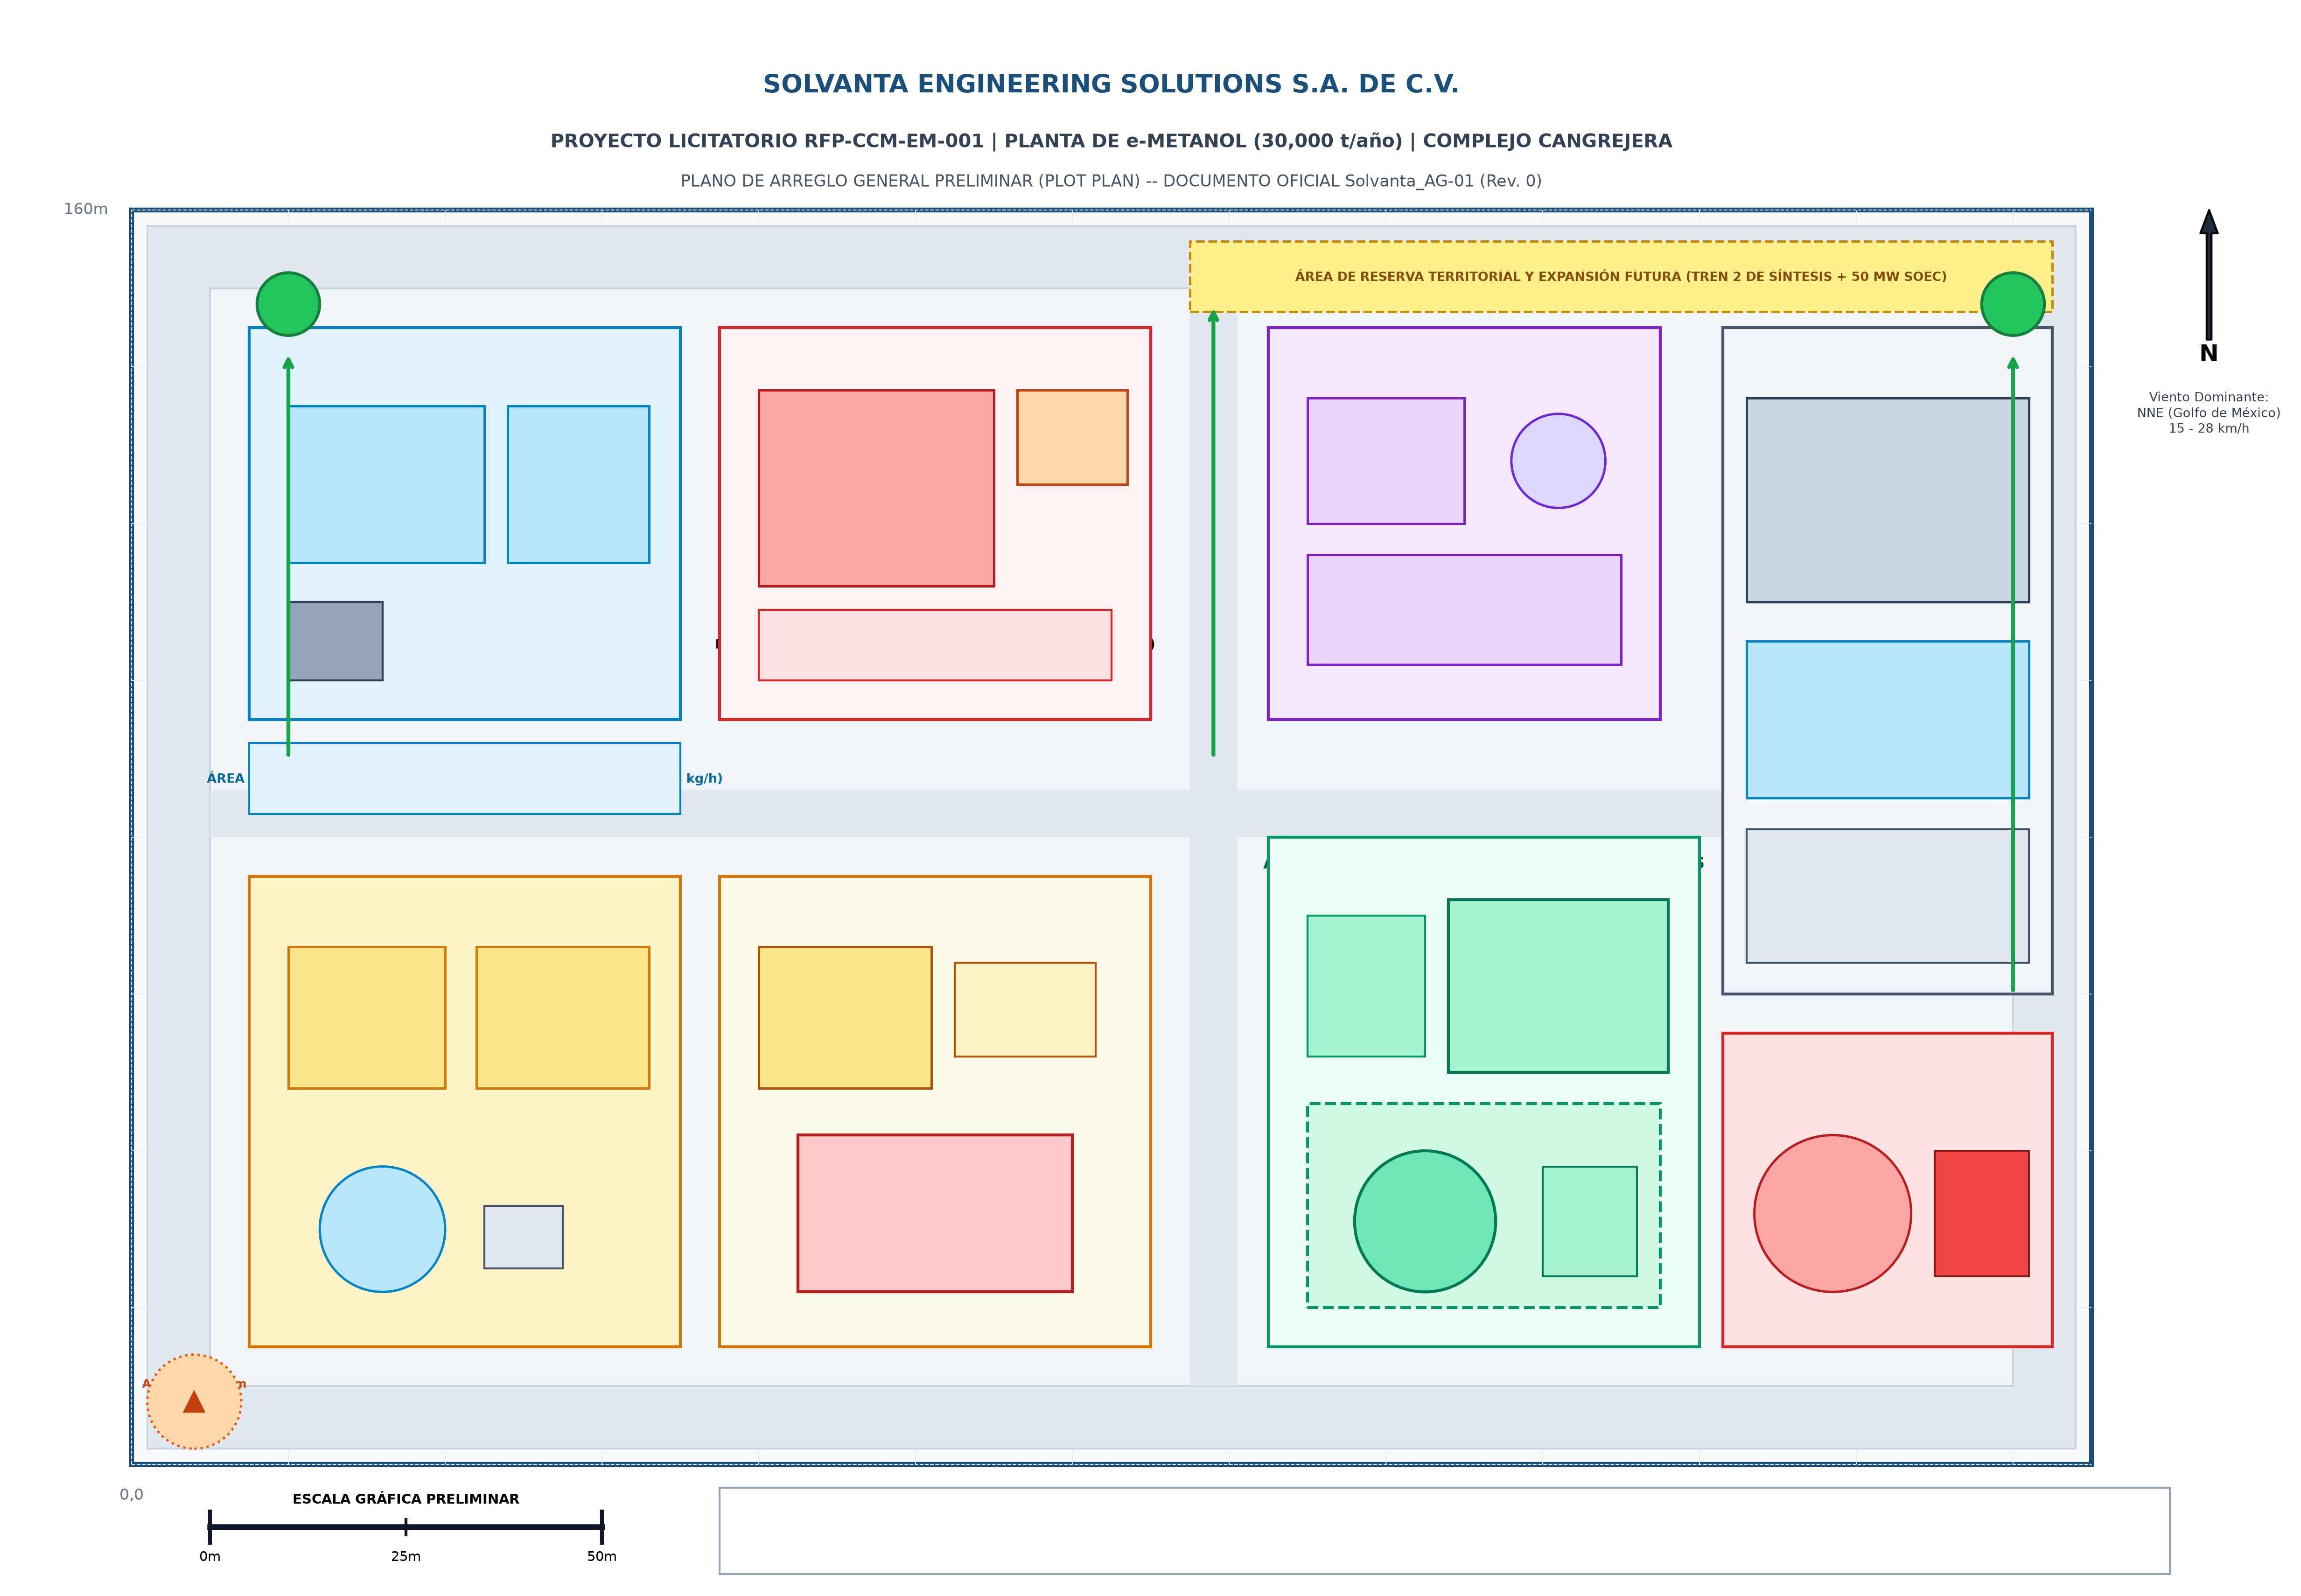
\includegraphics[width=0.96\linewidth]{figuras/Solvanta_AG-01.png}
    \caption{\textbf{Plano de Arreglo General Preliminar (Plot Plan) de la Planta de e-Metanol (Documento Solvanta\_AG-01 Rev. 0).}}
    \label{fig:plot_plan_oficial}
\end{figure}
\end{landscape}

\newpage
% ==============================================================================
% SECCIÓN 10: RESUMEN DEL TRATAMIENTO DEL HAZOP
% ==============================================================================
\section{Resumen del Tratamiento del HAZOP}

\subsection{Evolución del Diseño y Principales Hallazgos}
El taller HAZOP desarrollado por la firma \textbf{Solvanta Engineering Solutions} examinó exhaustivamente el diagrama preliminar congelado \textbf{DTI v0.2}, estructurándose en 10 nodos homogéneos de proceso. A lo largo del análisis se evaluaron \textbf{42 desviaciones creíbles} bajo condiciones normales, arranques transitorios, paros y fallas de servicios auxiliares.

El resultado del estudio demostró la robustez intrínseca del proceso, pero identificó cuatro riesgos mayores de severidad crítica que motivaron modificaciones inmediatas en la arquitectura de control, en la matriz de interbloqueos (\textbf{MI-01 Rev. 1}) y en las especificaciones mecánicas de los equipos:

\begin{enumerate}
    \item \textbf{Embalamiento Térmico en Reactor Tubular Lurgi \texttt{R-401} (Nodo 4):}
    \begin{itemize}
        \item \textit{Desviación y Escenario:} Temperatura muy alta por pérdida de agua de enfriamiento en la caldera \texttt{R-401-S} o disparo de la bomba \texttt{P-801}, lo que provoca rápida evaporación del inventario hídrico en la carcasa, acelerando la cinética exotérmica hasta alcanzar temperaturas superiores a $280^\circ\text{C}$ con riesgo de sinterización irreversible del catalizador de cobre y sobrepresión de tubos.
        \item \textit{Modificación Incorporada:} Se configuró el transmisor de temperatura múltiple \texttt{TT-401} con alarma simple de advertencia temprana \texttt{TAH-401} ($250^\circ\text{C}$) y el interbloqueo de seguridad \textbf{I-01} accionado por \texttt{TAHH-401} ($>260^\circ\text{C}$). Su activación dispara de forma instantánea el cierre estanco de la válvula \texttt{SDV-301} en la línea de gas fresco, abriendo simultáneamente el bypass del economizador \texttt{TV-502} y despresurizando parcialmente el bucle a través de la purga.
    \end{itemize}
    
    \item \textbf{Sobrepresión en el Bucle Cerrado de Síntesis a 75 bar (Nodos 4 y 5):}
    \begin{itemize}
        \item \textit{Desviación y Escenario:} Presión muy alta en bucle por bloqueo accidental de la válvula \texttt{LCV-501}, fallo en el soplador \texttt{C-501} o expansión térmica descontrolada, alcanzando la presión de diseño mecánico ($85.0\text{ bar}$).
        \item \textit{Modificación Incorporada:} Se incorporó el lazo \texttt{PIT-501} con alarma simple \texttt{PAH-501} ($76.5\text{ bar}$) para que el operador verifique el alineamiento del reciclo, y el interbloqueo \textbf{I-02} disparado por \texttt{PSHH-501} ($>78.5\text{ bar}$). Dicha función de seguridad detiene en seco los motores del compresor \texttt{C-301} y soplador \texttt{C-501}, abriendo la línea de recirculación anti-surge y aliviando el exceso de masa hacia el cabezal de antorcha mediante la válvula de alivio convencional \texttt{PSV-501} tarada a $80.0\text{ bar}$.
    \end{itemize}

    \item \textbf{Riesgo de Fractura en Membranas Cerámicas del Electrolizador SOEC \texttt{EL-201} (Nodo 2):}
    \begin{itemize}
        \item \textit{Desviación y Escenario:} Presión diferencial elevada entre la cámara catódica ($\text{H}_2/\text{H}_2\text{O}$) y la cámara anódica ($\text{O}_2$), provocada por fluctuación brusca en la línea de suministro de vapor o bloqueo en el cabezal de oxígeno. Un gradiente trans-membrana superior a $0.50\text{ bar}$ fractura mecánicamente el electrolito cerámico de circona estabilizada con itria (YSZ), generando mezcla explosiva $\text{H}_2/\text{O}_2$ a $800^\circ\text{C}$.
        \item \textit{Modificación Incorporada:} Se instaló transmisor de presión diferencial redundante \texttt{PDIT-201} con alarma simple temprana \texttt{PDAH-201} ($|\Delta P| > 0.30\text{ bar}$) que modula la válvula de venteo rápido de oxígeno \texttt{PDCV-201}, y el interbloqueo de disparo \textbf{I-03} activado por \texttt{PDAHH-201} ($>0.40\text{ bar}$), el cual corta instantáneamente la corriente eléctrica continua (DC) del rectificador de potencia, aislando el stack de celdas.
    \end{itemize}

    \item \textbf{Fenómeno de Gas Blow-by desde Separador Flash HP \texttt{V-501} hacia Flash LP \texttt{V-601} (Nodo 5 y 6):}
    \begin{itemize}
        \item \textit{Desviación y Escenario:} Nivel muy bajo en fondo de \texttt{V-501} provocado por fallo en apertura al $100\%$ de la válvula \texttt{LCV-501}. Al agotarse el sello hidráulico de líquido, el gas no convertido a $75.0\text{ bar}$ sopla directamente hacia el tambor desgasificador \texttt{V-601}, cuya presión de diseño es de sólo $6.0\text{ bar}$, provocando sobrepresión catastrófica y estallido mecánico del recipiente de baja presión.
        \item \textit{Modificación Incorporada:} Se implementó el transmisor de nivel independiente \texttt{LT-501} con alarma simple \texttt{LAL-501} ($20\%$) y el interbloqueo crítico \textbf{I-04} disparado por interruptor \texttt{LALL-501} ($10\%$). Esta lógica acciona el cierre estanco en menos de $1.0\text{ segundo}$ de la válvula de corte \textbf{\texttt{SDV-501}} (tipo Falla Cerrada, solenoide desenergizada), interrumpiendo el flujo antes de que el gas de alta presión invada el sistema de baja presión.
    \end{itemize}
\end{enumerate}

\subsection{Filosofía de Alarma Simple y Erradicación de Sobrediseño en Purgas}
Un aporte distintivo consolidado tras el HAZOP fue la adopción de una filosofía de ingeniería disciplinada que erradica el sobrediseño innecesario:
\begin{itemize}
    \item \textbf{Alarmas Simples y Directas:} Cada lazo de proceso cuenta con transmisores locales e indicadores en pantalla con alarmas auditivas y visuales intuitivas (\texttt{PAH/PAL}, \texttt{TAH/TAL}, \texttt{LAH/LAL}, \texttt{FAH/FAL}), asignando una consigna operativa clara antes de forzar el disparo del SIS.
    \item \textbf{Eliminación de Purgas Redundantes:} Se eliminaron líneas superfluas de blowdown y venteos continuos automáticos a antorcha. La \textbf{única purga de proceso conservada} es la corriente \textbf{S-505} ($613.59\text{ kg/h}$) hacia el turboexpansor \texttt{EXP-501}, estrictamente obligatoria por balance termodinámico para impedir la acumulación de metano y nitrógeno en el reciclo.
    \item \textbf{Válvulas Check en Descargas:} Se ratificó la instalación de válvulas antirretorno en todas las descargas de bombas (\texttt{P-201, P-601, P-602, P-801}) y compresores (\texttt{C-301, C-501}) para proteger sellos mecánicos contra contraflujos y golpes de ariete.
\end{itemize}

\subsection{Trazabilidad Documental y Acciones Abiertas}
La totalidad de las modificaciones físicas aprobadas quedaron registradas en el formato \textbf{RC-DTI-01} del expediente HAZOP y se trasladaron al catálogo maestro de equipos en \textbf{F-PIB-02C}. Las acciones de ingeniería que permanecen abiertas corresponden de manera transparente a los estudios tecno-económicos en BioSTEAM y a las memorias de dimensionamiento TEMA en HTRI, registradas formalmente en el formato \textbf{F-PIB-04} (asuntos TBD-01, TBD-02, HZ-01, HZ-02 y HZ-03).

\newpage
% ==============================================================================
% SECCIÓN 11: ORGANIZACIÓN DE LA FIRMA Y PLAN DE TRABAJO
% ==============================================================================
\section{Organización de la Firma y Plan de Trabajo}

\subsection{Asignación de Responsabilidades Técnicas}
En cumplimiento de la Sección 18 de la guía docente, los integrantes de la firma \textbf{Solvanta Engineering Solutions S.A. de C.V.} asumieron roles disciplinarios específicos para el desarrollo y verificación del Paquete de Ingeniería Básica PIB-01 (Cuadro \ref{tab:organizacion_firma}).

\begin{table}[H]
\centering\small
\setlength{\tabcolsep}{6pt}
\renewcommand{\arraystretch}{1.2}
\caption{\textbf{Organización sugerida de la firma y responsabilidades técnicas.}} \label{tab:organizacion_firma}
\begin{tabularx}{\textwidth}{>{\bfseries}p{3.5cm} p{4.2cm} X >{\bfseries}p{3.2cm}}
\toprule
\rowcolor{tableheader}
\color{white}\textbf{Función en el PIB} & \color{white}\textbf{Responsabilidad Principal} & \color{white}\textbf{Ingeniero(a) Responsable} & \color{white}\textbf{Evidencia Generada} \\
\midrule
Coordinación General & Control de alcance, calidad documental, gestión de revisiones y emisión del expediente integrado. & Ing. Karol Paola Camacho López (Directora de Proyecto) & Portada, control documental y F-PIB-01 \\ \addlinespace[2pt]
Ingeniería de Proceso & Consolidar bases de proceso, inventario de los 30 equipos y redactar memoria descriptiva. & Ing. Paulina Mota Macip (Especialista en Simulación) & F-PIB-01, F-PIB-02 y Memoria Descriptiva \\ \addlinespace[2pt]
Servicios y Balances & Consolidar balance riguroso de materias primas, servicios y salidas con cálculo anualizado. & Ing. Grecia Figueroa Rincón (Especialista en HSE y Balances) & F-PIB-03 y cálculos anualizados en LaTeX \\ \addlinespace[2pt]
Seguridad y Control & Verificar la incorporación de hallazgos HAZOP, matriz MCE-01 Rev. 1 e interbloqueos mayores. & Ing. Grecia Figueroa Rincón \& Ing. Paulina Mota Macip & Resumen HAZOP y catálogo de salvaguardas \\ \addlinespace[2pt]
Distribución Espacial & Desarrollar el plano de Arreglo General Preliminar (Plot Plan) con distancias y zonas seguras. & Ing. Gildardo Ocaña Barrales (Custodio DTI / Plant 3D) & Plano oficial Solvanta\_AG-01 \\ \addlinespace[2pt]
Verificación y Calidad & Identificar y documentar exhaustivamente datos pendientes, inconsistencias y plan de cierre. & Ing. Karol Paola Camacho López \& Ing. Gildardo Ocaña Barrales & Formato F-PIB-04 y Acta de Auditoría \\
\bottomrule
\end{tabularx}
\end{table}

\subsection{Cronograma de Trabajo Desarrollado}
Las actividades del paquete de ingeniería se ejecutaron a través de seis sesiones técnicas estructuradas:
\begin{enumerate}
    \item \textbf{Sesión 1 (Congelamiento Documental):} Registro y verificación de versiones de DWSIM v1, LE-01 Rev. 1, DTI v0.2 y AC-HAZOP-01. Asignación de responsabilidades.
    \item \textbf{Sesión 2 (Consolidación de Bases):} Formulación de F-PIB-01, cálculo de disponibilidad ($91.32\%$) y producción anual ($30\,309.20\text{ t/año}$).
    \item \textbf{Sesión 3 (Inventario de Equipos):} Elaboración de F-PIB-02 (Partes A, B y C), clasificación de variables de tamaño y distinción entre potencias y cargas térmicas.
    \item \textbf{Sesión 4 (Balance de Recursos y Servicios):} Elaboración de F-PIB-03 (Partes A y B), desglose de energía eléctrica ($39.10\text{ MWe}$ optimizados en Escenario D), agua de enfriamiento circulante ($2\,218.4\text{ m}^3\text{/h}$) vs reposición ($33.3\text{ m}^3\text{/h}$) y vapor.
    \item \textbf{Sesión 5 (Integración y Memoria Descriptiva):} Redacción de la memoria descriptiva en 17 puntos y modelado del plano de Arreglo General Preliminar Solvanta\_AG-01.
    \item \textbf{Sesión 6 (Auditoría, Pendientes y Cierre):} Consolidación de F-PIB-04, auditoría técnica cruzada y compilación del expediente final PIB-01.
\end{enumerate}

\newpage
% ==============================================================================
% SECCIÓN 12: LISTA DE VERIFICACIÓN FORMAL
% ==============================================================================
\section{Lista de Verificación Formal de la Firma Solvanta}

En cumplimiento de la Sección 19 de la guía docente, la firma auditó cada uno de los criterios técnicos antes de autorizar la emisión de la Revisión 0 del expediente (Cuadro \ref{tab:lista_verificacion}).

\begin{table}[H]
\centering\small
\setlength{\tabcolsep}{5pt}
\renewcommand{\arraystretch}{1.15}
\caption{\textbf{Lista de verificación técnica oficial de PIB-01.}} \label{tab:lista_verificacion}
\begin{tabularx}{\textwidth}{c X c p{5.5cm}}
\toprule
\rowcolor{tableheader}
\color{white}\textbf{Núm.} & \color{white}\textbf{Criterio de Verificación Técnica de la Guía} & \color{white}\textbf{Estado} & \color{white}\textbf{Evidencia Verificable en Solvanta-PIB-01} \\
\midrule
1 & Se identificó la revisión de todos los documentos utilizados. & \textbf{[X]} Sí & Sección 1.5 detalla revisiones oficiales congeladas. \\
2 & Las capacidades de F-PIB-01 coinciden con las Bases de Diseño. & \textbf{[X]} Sí & $3\,788.65\text{ kg/h}$ ($30\,309.20\text{ t/año}$) en Cuadro \ref{tab:fpib01}. \\
3 & Las horas de operación están justificadas. & \textbf{[X]} Sí & $8\,000\text{ h/año}$ justificadas en Sección 2.2.1. \\
4 & La producción anual fue calculada correctamente. & \textbf{[X]} Sí & Operación matemática explícita en Sección 2.2.2. \\
5 & Los límites de batería están definidos. & \textbf{[X]} Sí & Parámetros BD-10 y BD-11 en Cuadro \ref{tab:fpib01}. \\
6 & Todos los equipos principales aparecen en F-PIB-02. & \textbf{[X]} Sí & Censo de los 30 equipos en Cuadros \ref{tab:fpib02a}, \ref{tab:fpib02b} y \ref{tab:fpib02c}. \\
7 & Los tags coinciden con PFD y DTI. & \textbf{[X]} Sí & Concordancia estricta de tags (\texttt{EL-201, C-301, R-401, T-601}). \\
8 & Las capacidades normales y máximas tienen unidades. & \textbf{[X]} Sí & Expresadas con unidades (kg/h, m³/h, t/h). \\
9 & Presiones y temperaturas coinciden con DWSIM v1. & \textbf{[X]} Sí & Verificadas contra convergencia termodinámica PRSV2-VL. \\
10 & Cada equipo tiene una variable de tamaño identificada. & \textbf{[X]} Sí & Columna específica en Cuadro \ref{tab:fpib02b}. \\
11 & Se distinguió potencia de carga térmica. & \textbf{[X]} Sí & Diferenciación rigurosa de kW mec./eléc. vs kW térmicos. \\
12 & Los materiales no confirmados se registraron como TBD o preliminar. & \textbf{[X]} Sí & Clasificados con norma ASTM/ASME preliminar en F-PIB-02B. \\
13 & Los requisitos HAZOP se vincularon con los equipos. & \textbf{[X]} Sí & Detallados para cada equipo en Cuadro \ref{tab:fpib02c}. \\
14 & Las materias primas aparecen en F-PIB-03. & \textbf{[X]} Sí & $\text{CO}_2$ ($42\,194.7\text{ t/año}$) y agua fresca ($73\,934.7\text{ t/año}$). \\
15 & Los servicios auxiliares aparecen en F-PIB-03. & \textbf{[X]} Sí & Electricidad, vapor, agua de enfriamiento, chilled water, N2. \\
16 & Los productos y subproductos están registrados. & \textbf{[X]} Sí & e-Metanol Grado AA, oxígeno medicinal, gas de purga. \\
17 & Los residuos y efluentes están registrados. & \textbf{[X]} Sí & Salmuera concentrada ZLD y venteo de ligeros flash LP. \\
18 & Las cantidades anuales tienen cálculo o fuente. & \textbf{[X]} Sí & Fórmulas explícitas en Sección 4.2 y Cuadro \ref{tab:fpib03b}. \\
19 & Se distinguió flujo circulante de flujo de reposición. & \textbf{[X]} Sí & Circulante CW ($2\,218.4\text{ m}^3\text{/h}$) vs make-up ($33.3\text{ m}^3\text{/h}$). \\
20 & La memoria descriptiva coincide con los diagramas. & \textbf{[X]} Sí & Articulada en 17 puntos y cuadro por secciones 100-800. \\
21 & El arreglo general identifica las áreas principales. & \textbf{[X]} Sí & Plano Solvanta\_AG-01 con las 16 zonas requeridas. \\
22 & Las decisiones derivadas del HAZOP están resumidas. & \textbf{[X]} Sí & Resumen en Sección 7 con 4 interlocks mayores (I-01 a I-04). \\
23 & Todos los datos faltantes aparecen en F-PIB-04. & \textbf{[X]} Sí & Cuadro \ref{tab:fpib04a} con 12 asuntos (TBD, INC, HZ, OT). \\
24 & Cada pendiente tiene acción y responsable. & \textbf{[X]} Sí & Asignados con nombre, fecha y evidencia en Cuadro \ref{tab:fpib04b}. \\
25 & Las inconsistencias fueron corregidas o permanecen documentadas. & \textbf{[X]} Sí & INC-01, INC-02 e INC-03 resueltas con evidencia de cierre. \\
26 & Una persona diferente al elaborador realizó la revisión. & \textbf{[X]} Sí & Auditoría cruzada plasmada en el Acta de Verificación. \\
27 & El expediente no contiene cálculos económicos. & \textbf{[X]} Sí & Exclusión total de costos, CAPEX, OPEX y rentabilidad. \\
\bottomrule
\end{tabularx}
\end{table}

\newpage
% ==============================================================================
% SECCIÓN 13: ACTA BREVE DE REVISIÓN CRUZADA
% ==============================================================================
\section{Acta Breve de Revisión Cruzada de la Firma}

En cumplimiento de los requisitos de aseguramiento de calidad de la firma \textbf{Solvanta Engineering Solutions S.A. de C.V.}, se certifica formalmente que los documentos, formatos de cálculo y planos que integran el presente Paquete de Ingeniería Básica PIB-01 fueron sometidos a una auditoría técnica independiente y cruzada, en la que cada sección fue revisada por un ingeniero distinto a quien la elaboró (Cuadro \ref{tab:acta_cruzada}).

\begin{table}[H]
\centering\small
\setlength{\tabcolsep}{6pt}
\renewcommand{\arraystretch}{1.2}
\caption{\textbf{Acta oficial de revisión técnica cruzada y conformidad de ingeniería.}} \label{tab:acta_cruzada}
\begin{tabularx}{\textwidth}{p{3.5cm} p{4.2cm} p{4.2cm} >{\raggedright\arraybackslash}X}
\toprule
\rowcolor{tableheader}
\color{white}\textbf{Sección / Formato} & \color{white}\textbf{Ingeniero Elaborador} & \color{white}\textbf{Ingeniero Revisor Cruzado} & \color{white}\textbf{Dictamen Técnico} \\
\midrule
F-PIB-01 (Bases consolidadas) & Ing. Karol Paola Camacho López & Ing. Paulina Mota Macip & \textit{Conforme --- Coincidencia absoluta con DWSIM v1 y RFP-CCM-EM-001.} \\ \addlinespace[2pt]
F-PIB-02 (Inventario equipos) & Ing. Paulina Mota Macip & Ing. Gildardo Ocaña Barrales & \textit{Conforme --- 30 equipos verificados con DFP v1 y DTI v0.2.} \\ \addlinespace[2pt]
F-PIB-03 (Recursos y servicios) & Ing. Grecia Figueroa Rincón & Ing. Paulina Mota Macip & \textit{Conforme --- Cálculos anuales en LaTeX validados con TE-01.} \\ \addlinespace[2pt]
F-PIB-04 (Pendientes y verificación) & Ing. Karol Paola Camacho López & Ing. Gildardo Ocaña Barrales & \textit{Conforme --- 12 asuntos trazados con responsable y evidencia.} \\ \addlinespace[2pt]
Memoria descriptiva & Ing. Paulina Mota Macip & Ing. Karol Paola Camacho López & \textit{Conforme --- 17 puntos desarrollados y consistentes.} \\ \addlinespace[2pt]
Arreglo general Solvanta\_AG-01 & Ing. Gildardo Ocaña Barrales & Ing. Grecia Figueroa Rincón & \textit{Conforme --- Cumplimiento estricto de distancias NFPA/API.} \\ \addlinespace[2pt]
Resumen HAZOP y salvaguardas & Ing. Grecia Figueroa Rincón & Ing. Karol Paola Camacho López & \textit{Conforme --- Interlocks I-01 a I-04 consistentes con MCE-01.} \\
\bottomrule
\end{tabularx}
\end{table}

\vspace{0.8cm}
\begin{center}
\small
\setlength{\tabcolsep}{12pt}
\begin{tabular}{cc}
\textbf{Ing. Karol Paola Camacho López} & \textbf{Ing. Paulina Mota Macip} \\
Directora de Proyecto \textbar\ Coordinación & Especialista en Simulación y Proceso \\[0.8cm]
\textbf{Ing. Gildardo Ocaña Barrales} & \textbf{Ing. Grecia Figueroa Rincón} \\
Custodio del DTI \textbar\ Arreglo General & Especialista en Seguridad y HSE \\
\end{tabular}
\end{center}

\newpage
% ==============================================================================
% SECCIÓN 14: ANEXOS TÉCNICOS OFICIALES
% ==============================================================================
\section{Anexos Técnicos Oficiales}

\subsection{Anexo A: Tabla Oficial de Corrientes de Proceso (TC-01)}
A continuación se incorpora el balance completo de materia y condiciones termodinámicas para las 36 corrientes del proceso, procedente de la convergencia oficial de \texttt{DWSIM v1} (Cuadros \ref{tab:tc01a_anexo} y \ref{tab:tc01b_anexo}).

\begin{landscape}
\footnotesize
\setlength{\tabcolsep}{3.5pt}
\begin{xltabular}{\linewidth}{|l|p{6.0cm}|c|r|r|r|r|c|}
\caption{\textbf{Anexo A: Tabla Oficial de Corrientes de Proceso TC-01A (Propiedades Termodinámicas).}} \label{tab:tc01a_anexo} \\ \hline
\rowcolor{tableheader}\color{white}\textbf{ID} & \color{white}\textbf{Descripción de Tubería / Tramo de Proceso} & \color{white}\textbf{Fase} & \color{white}\textbf{Temp. ($^\circ$C)} & \color{white}\textbf{Presión (bar)} & \color{white}\textbf{Flujo Másico (kg/h)} & \color{white}\textbf{Flujo Molar (kmol/h)} & \color{white}\textbf{Frac. Vap.} \\ \hline
\endfirsthead
\multicolumn{8}{c}{\footnotesize\textit{Continuación del Cuadro \ref{tab:tc01a_anexo} - Tabla TC-01A}} \\ \hline
\rowcolor{tableheader}\color{white}\textbf{ID} & \color{white}\textbf{Descripción de Tubería / Tramo de Proceso} & \color{white}\textbf{Fase} & \color{white}\textbf{Temp. ($^\circ$C)} & \color{white}\textbf{Presión (bar)} & \color{white}\textbf{Flujo Másico (kg/h)} & \color{white}\textbf{Flujo Molar (kmol/h)} & \color{white}\textbf{Frac. Vap.} \\ \hline
\endhead
\hline \multicolumn{8}{r}{\footnotesize\textit{Continúa en la siguiente página...}} \\
\endfoot
\hline
\endlastfoot
S-101 & Alimentación $\text{CO}_2$ de captura externa & Vapor & 25.0 & 20.00 & 5\,274.34 & 121.000 & 1.00 \\ \hline
S-201 & Agua make-up fresca de red & Líquido & 25.0 & 20.00 & 9\,241.84 & 513.000 & 0.00 \\ \hline
S-202 & Retorno agua tratada circuito ZLD & Líquido & 59.2 & 20.00 & 7\,003.86 & 388.768 & 0.00 \\ \hline
S-203 & Agua combinada de caldera a R-401-S & Líquido & 39.8 & 20.00 & 16\,244.88 & 901.722 & 0.00 \\ \hline
S-204 & Vapor saturado 20 bar generado en caldera & Vapor & 220.0 & 20.00 & 16\,244.88 & 901.722 & 1.00 \\ \hline
S-205 & Vapor sobrecalentado a 800 $^\circ$C a SOEC & Vapor & 800.0 & 20.00 & 16\,244.88 & 901.722 & 1.00 \\ \hline
S-206 & Oxígeno puro SOEC (ánodo) & Vapor & 31.0 & 19.40 & 10\,098.76 & 315.598 & 1.00 \\ \hline
S-207 & Efluente húmedo SOEC (cátodo) & Vapor & 800.0 & 19.40 & 6\,145.79 & 901.712 & 1.00 \\ \hline
S-208 & Efluente SOEC enfriado bifásico & Bifásica & 38.0 & 19.40 & 6\,145.79 & 901.712 & 0.70 \\ \hline
S-209 & Hidrógeno verde seco puro a síntesis & Vapor & 38.0 & 19.40 & 1\,314.77 & 633.548 & 1.00 \\ \hline
S-210 & Condensado SOEC no disociado a ZLD & Líquido & 38.0 & 19.40 & 4\,831.02 & 268.165 & 0.00 \\ \hline
S-301 & Syngas fresco combinado ($M=2.05$) & Vapor & 32.9 & 19.40 & 6\,589.11 & 754.548 & 1.00 \\ \hline
S-302 & Syngas precalentado a succión C-301 & Vapor & 71.7 & 19.40 & 6\,589.11 & 754.548 & 1.00 \\ \hline
S-303 & Syngas comprimido a 75 bar de descarga & Vapor & 271.0 & 75.00 & 6\,589.11 & 754.548 & 1.00 \\ \hline
S-401 & Alimentación total combinada a reactor R-401 & Vapor & 83.2 & 75.00 & 21\,308.08 & 7\,387.096 & 1.00 \\ \hline
S-402 & Efluente reactivo síntesis de metanol & Vapor & 245.0 & 75.00 & 21\,308.08 & 7\,149.098 & 1.00 \\ \hline
S-403 & Efluente economizado tras FEHE E-502 & Vapor & 224.6 & 75.00 & 21\,308.08 & 7\,149.098 & 1.00 \\ \hline
S-404 & Efluente condensado bifásico a V-501 & Bifásica & 38.0 & 75.00 & 21\,308.08 & 7\,149.098 & 0.97 \\ \hline
S-501 & Gas en domo de flash HP V-501 & Vapor & 38.0 & 75.00 & 15\,339.75 & 6\,909.568 & 1.00 \\ \hline
S-502 & Gas bucle sobrecalentado & Vapor & 60.0 & 75.00 & 15\,339.75 & 6\,909.568 & 1.00 \\ \hline
S-503 & Gas de reciclo circulante ($96\%$) & Vapor & 60.0 & 75.00 & 14\,726.16 & 6\,633.185 & 1.00 \\ \hline
S-504\_OUT & Gas de reciclo impulsado por C-501 & Vapor & 60.0 & 75.00 & 14\,726.16 & 6\,633.185 & 1.00 \\ \hline
S-505 & Gas de purga continua de inertes ($4\%$) & Vapor & 60.0 & 75.00 & 613.59 & 276.383 & 1.00 \\ \hline
S-506 & Purga expandida tras turboexpansor & Bifásica & -138.6 & 1.10 & 613.59 & 276.383 & 1.00 \\ \hline
S-507 & Metanol crudo líquido fondo flash HP & Líquido & 38.0 & 75.00 & 5\,968.39 & 239.530 & 0.00 \\ \hline
S-507A & Metanol crudo tras válvula JT a 1.25 bar & Bifásica & 38.0 & 1.25 & 5\,968.39 & 239.530 & 0.01 \\ \hline
S-601 & Venteo gases disueltos flash LP & Bifásica & 38.0 & 1.25 & 6.57 & 0.556 & 0.91 \\ \hline
S-602 & Metanol crudo desgasificado a bomba & Líquido & 38.0 & 1.25 & 5\,961.82 & 238.975 & 0.00 \\ \hline
S-602A & Metanol crudo presurizado a plato 18 & Líquido & 38.0 & 2.20 & 5\,961.82 & 238.975 & 0.00 \\ \hline
S-603 & Vapores de metanol en domo de torre & Líquido & 68.5 & 1.20 & 3\,788.65 & 118.341 & 0.00 \\ \hline
\textbf{S-604} & \textbf{e-Metanol Grado Químico AA Comercial} & \textbf{Líquido} & \textbf{35.0} & \textbf{1.10} & \textbf{3\,788.65} & \textbf{118.341} & \textbf{0.00} \\ \hline
S-605 & Fondos acuosos despojados de torre & Líquido & 103.9 & 1.25 & 2\,173.40 & 120.634 & 0.00 \\ \hline
S-801 & Efluente hídrico combinado a ZLD & Líquido & 58.9 & 1.25 & 7\,004.41 & 388.798 & 0.00 \\ \hline
S-802 & Agua clarificada y filtrada ZLD & Líquido & 58.9 & 1.25 & 7\,004.41 & 388.798 & 0.00 \\ \hline
S-803 & Agua desmineralizada presurizada a caldera & Líquido & 59.2 & 20.00 & 7\,004.41 & 388.798 & 0.00 \\ \hline
S-804 & Purga lodos salinos concentrados ZLD & Líquido & 58.9 & 1.25 & 0.56 & 0.030 & 0.00 \\ \hline
\end{xltabular}
\end{landscape}

\newpage
\begin{landscape}
\footnotesize
\setlength{\tabcolsep}{5pt}
\begin{xltabular}{\linewidth}{|l|c|c|c|c|c|c|c|}
\caption{\textbf{Anexo A (Cont.): Tabla Oficial de Corrientes TC-01B (Composiciones Molares Exactas).}} \label{tab:tc01b_anexo} \\ \hline
\rowcolor{tableheader}\color{white}\textbf{ID Corriente} & \color{white}\textbf{$x_{\text{CO}_2}$} & \color{white}\textbf{$x_{\text{CO}}$} & \color{white}\textbf{$x_{\text{H}_2}$} & \color{white}\textbf{$x_{\text{H}_2\text{O}}$} & \color{white}\textbf{$x_{\text{MeOH}}$} & \color{white}\textbf{$x_{\text{O}_2}$} & \color{white}\textbf{$\sum x_i$} \\ \hline
\endfirsthead
\multicolumn{8}{c}{\footnotesize\textit{Continuación del Cuadro \ref{tab:tc01b_anexo} - Tabla TC-01B}} \\ \hline
\rowcolor{tableheader}\color{white}\textbf{ID Corriente} & \color{white}\textbf{$x_{\text{CO}_2}$} & \color{white}\textbf{$x_{\text{CO}}$} & \color{white}\textbf{$x_{\text{H}_2}$} & \color{white}\textbf{$x_{\text{H}_2\text{O}}$} & \color{white}\textbf{$x_{\text{MeOH}}$} & \color{white}\textbf{$x_{\text{O}_2}$} & \color{white}\textbf{$\sum x_i$} \\ \hline
\endhead
\hline \multicolumn{8}{r}{\footnotesize\textit{Continúa en la siguiente página...}} \\
\endfoot
\hline
\endlastfoot
S-101 & 0.9900 & 0.0000 & 0.0100 & 0.0000 & 0.0000 & 0.0000 & 1.0000 \\ \hline
S-201 & 0.0000 & 0.0000 & 0.0000 & 1.0000 & 0.0000 & 0.0000 & 1.0000 \\ \hline
S-202 & 0.0000 & 0.0000 & 0.0000 & 1.0000 & 0.0000 & 0.0000 & 1.0000 \\ \hline
S-203 & 0.0000 & 0.0000 & 0.0000 & 1.0000 & 0.0000 & 0.0000 & 1.0000 \\ \hline
S-204 & 0.0000 & 0.0000 & 0.0000 & 1.0000 & 0.0000 & 0.0000 & 1.0000 \\ \hline
S-205 & 0.0000 & 0.0000 & 0.0000 & 1.0000 & 0.0000 & 0.0000 & 1.0000 \\ \hline
S-206 & 0.0000 & 0.0000 & 0.0000 & 0.0000 & 0.0000 & 1.0000 & 1.0000 \\ \hline
S-207 & 0.0000 & 0.0000 & 0.7000 & 0.3000 & 0.0000 & 0.0000 & 1.0000 \\ \hline
S-208 & 0.0000 & 0.0000 & 0.7000 & 0.3000 & 0.0000 & 0.0000 & 1.0000 \\ \hline
S-209 & 0.0000 & 0.0000 & 0.9963 & 0.0037 & 0.0000 & 0.0000 & 1.0000 \\ \hline
S-210 & 0.0000 & 0.0000 & 0.0000 & 1.0000 & 0.0000 & 0.0000 & 1.0000 \\ \hline
S-301 & 0.1588 & 0.0000 & 0.8381 & 0.0031 & 0.0000 & 0.0000 & 1.0000 \\ \hline
S-302 & 0.1588 & 0.0000 & 0.8381 & 0.0031 & 0.0000 & 0.0000 & 1.0000 \\ \hline
S-303 & 0.1588 & 0.0000 & 0.8381 & 0.0031 & 0.0000 & 0.0000 & 1.0000 \\ \hline
S-401 & 0.0183 & 0.0000 & 0.9776 & 0.0016 & 0.0025 & 0.0000 & 1.0000 \\ \hline
S-402 & 0.0023 & 0.0000 & 0.9603 & 0.0183 & 0.0192 & 0.0000 & 1.0000 \\ \hline
S-403 & 0.0023 & 0.0000 & 0.9603 & 0.0183 & 0.0192 & 0.0000 & 1.0000 \\ \hline
S-404 & 0.0023 & 0.0000 & 0.9603 & 0.0183 & 0.0192 & 0.0000 & 1.0000 \\ \hline
S-501 & 0.0023 & 0.0000 & 0.9935 & 0.0014 & 0.0028 & 0.0000 & 1.0000 \\ \hline
S-502 & 0.0023 & 0.0000 & 0.9935 & 0.0014 & 0.0028 & 0.0000 & 1.0000 \\ \hline
S-503 & 0.0023 & 0.0000 & 0.9935 & 0.0014 & 0.0028 & 0.0000 & 1.0000 \\ \hline
S-504\_OUT & 0.0023 & 0.0000 & 0.9935 & 0.0014 & 0.0028 & 0.0000 & 1.0000 \\ \hline
S-505 & 0.0023 & 0.0000 & 0.9935 & 0.0014 & 0.0028 & 0.0000 & 1.0000 \\ \hline
S-506 & 0.0023 & 0.0000 & 0.9935 & 0.0014 & 0.0028 & 0.0000 & 1.0000 \\ \hline
S-507 & 0.0004 & 0.0000 & 0.0017 & 0.5046 & 0.4933 & 0.0000 & 1.0000 \\ \hline
S-507A & 0.0004 & 0.0000 & 0.0017 & 0.5046 & 0.4933 & 0.0000 & 1.0000 \\ \hline
S-601 & 0.1729 & 0.0000 & 0.7420 & 0.0000 & 0.0850 & 0.0000 & 1.0000 \\ \hline
S-602 & 0.0000 & 0.0000 & 0.0000 & 0.5058 & 0.4942 & 0.0000 & 1.0000 \\ \hline
S-602A & 0.0000 & 0.0000 & 0.0000 & 0.5058 & 0.4942 & 0.0000 & 1.0000 \\ \hline
S-603 & 0.0000 & 0.0000 & 0.0000 & 0.0019 & 0.9981 & 0.0000 & 1.0000 \\ \hline
\textbf{S-604} & \textbf{0.0000} & \textbf{0.0000} & \textbf{0.0000} & \textbf{0.0019} & \textbf{0.9981} & \textbf{0.0000} & \textbf{1.0000} \\ \hline
S-605 & 0.0000 & 0.0000 & 0.0000 & 0.9999 & 0.0001 & 0.0000 & 1.0000 \\ \hline
S-801 & 0.0000 & 0.0000 & 0.0000 & 1.0000 & 0.0000 & 0.0000 & 1.0000 \\ \hline
S-802 & 0.0000 & 0.0000 & 0.0000 & 1.0000 & 0.0000 & 0.0000 & 1.0000 \\ \hline
S-803 & 0.0000 & 0.0000 & 0.0000 & 1.0000 & 0.0000 & 0.0000 & 1.0000 \\ \hline
S-804 & 0.0000 & 0.0000 & 0.0180 & 0.9819 & 0.0001 & 0.0000 & 1.0000 \\ \hline
\end{xltabular}
\end{landscape}

\newpage
\subsection{Anexo B: Tabla Oficial de Energía y Servicios (TE-01)}
El Cuadro \ref{tab:te01_anexo} resume las cargas térmicas y demandas eléctricas unitarias procedentes de \texttt{DWSIM v1}.

\begin{table}[H]
\centering\small
\setlength{\tabcolsep}{4pt}
\renewcommand{\arraystretch}{1.15}
\caption{\textbf{Anexo B: Tabla Oficial de Energía y Servicios TE-01.}} \label{tab:te01_anexo}
\begin{tabularx}{\textwidth}{l p{2.8cm} p{4.0cm} c r r r}
\toprule
\rowcolor{tableheader}
\color{white}\textbf{Tag} & \color{white}\textbf{Servicio} & \color{white}\textbf{Descripción del Equipo} & \color{white}\textbf{$T_{\text{in}} \to T_{\text{out}}$} & \color{white}\textbf{$Q$ (kW)} & \color{white}\textbf{$W$ (kW)} & \color{white}\textbf{MWh/año} \\
\midrule
\texttt{EL-201} & Electricidad AC/DC & Stack electrólisis SOEC vapor & 800 $\to$ 800 & --- & +38\,067.30 & 304\,538.4 \\
\texttt{E-202} & Calef. eléctrica & Sobrecalentador vapor SOEC & 220 $\to$ 800 & +5\,248.42 & --- & 41\,987.4 \\
\texttt{E-203} & Agua enfriam. & Condensador efluente SOEC & 800 $\to$ 38 & -8\,962.22 & --- & 71\,697.8 \\
\texttt{E-301} & Calefacción LP & Precalentador syngas fresco & 33 $\to$ 72 & +250.00 & --- & 2\,000.0 \\
\texttt{C-301} & Electricidad & Compresor syngas multietapa & 72 $\to$ 271 & --- & +1\,316.67 & 10\,533.4 \\
\texttt{R-401-S} & Gen. vapor 20 bar & Carcasa caldera acoplada & 40 $\to$ 220 & -12\,335.36 & --- & 98\,682.9 \\
\texttt{R-401} & Reacción exotérm. & Reactor tubular Lurgi BWR & 245 $\to$ 245 & -7\,924.76 & --- & 63\,398.1 \\
\texttt{E-502A/B} & Integración térm. & Economizador FEHE bucle & 245 $\to$ 225 & +1\,235.43 & --- & 9\,883.4 \\
\texttt{E-501} & Agua enfriam. & Condensador bucle síntesis & 225 $\to$ 38 & -13\,742.75 & --- & 109\,942.0 \\
\texttt{C-501} & Electricidad & Soplador centrífugo reciclo & 60 $\to$ 60 & --- & +150.00 & 1\,200.0 \\
\texttt{EXP-501} & Generación eléc. & Turboexpansor gas purga & 60 $\to$ -139 & --- & -437.79 & -3\,502.3 \\
\texttt{E-601} & Agua enfriam. & Condensador domo torre T-601 & 68.5 $\to$ 68.5 & -3\,077.25 & --- & 24\,618.0 \\
\texttt{E-602} & Vapor 3.5 bar & Rehervidor fondos torre T-601 & 104 $\to$ 104 & +3\,266.68 & --- & 26\,133.4 \\
\texttt{E-603} & Agua helada & Subenfriador metanol Grado AA & 68.5 $\to$ 35 & -111.11 & --- & 888.9 \\
\texttt{Bombas} & Electricidad & Bombas auxiliares (P-201/601/602/801) & Varios & --- & +14.63 & 117.0 \\
\midrule
\multicolumn{4}{l}{\textbf{Demanda Eléctrica Neta Global de Planta}} & --- & $\mathbf{+39\,101.69}$ & $\mathbf{312\,813.5}$ \\
\bottomrule
\end{tabularx}
\end{table}

\subsection{Anexo C: Diagrama de Tuberías e Instrumentación (DTI v0.2 / DTI v1)}
A continuación se incorpora en hoja apaisada la lámina oficial del plano de tuberías e instrumentación analizado en el taller HAZOP, con base en el cual se integró el presente Paquete de Ingeniería Básica.

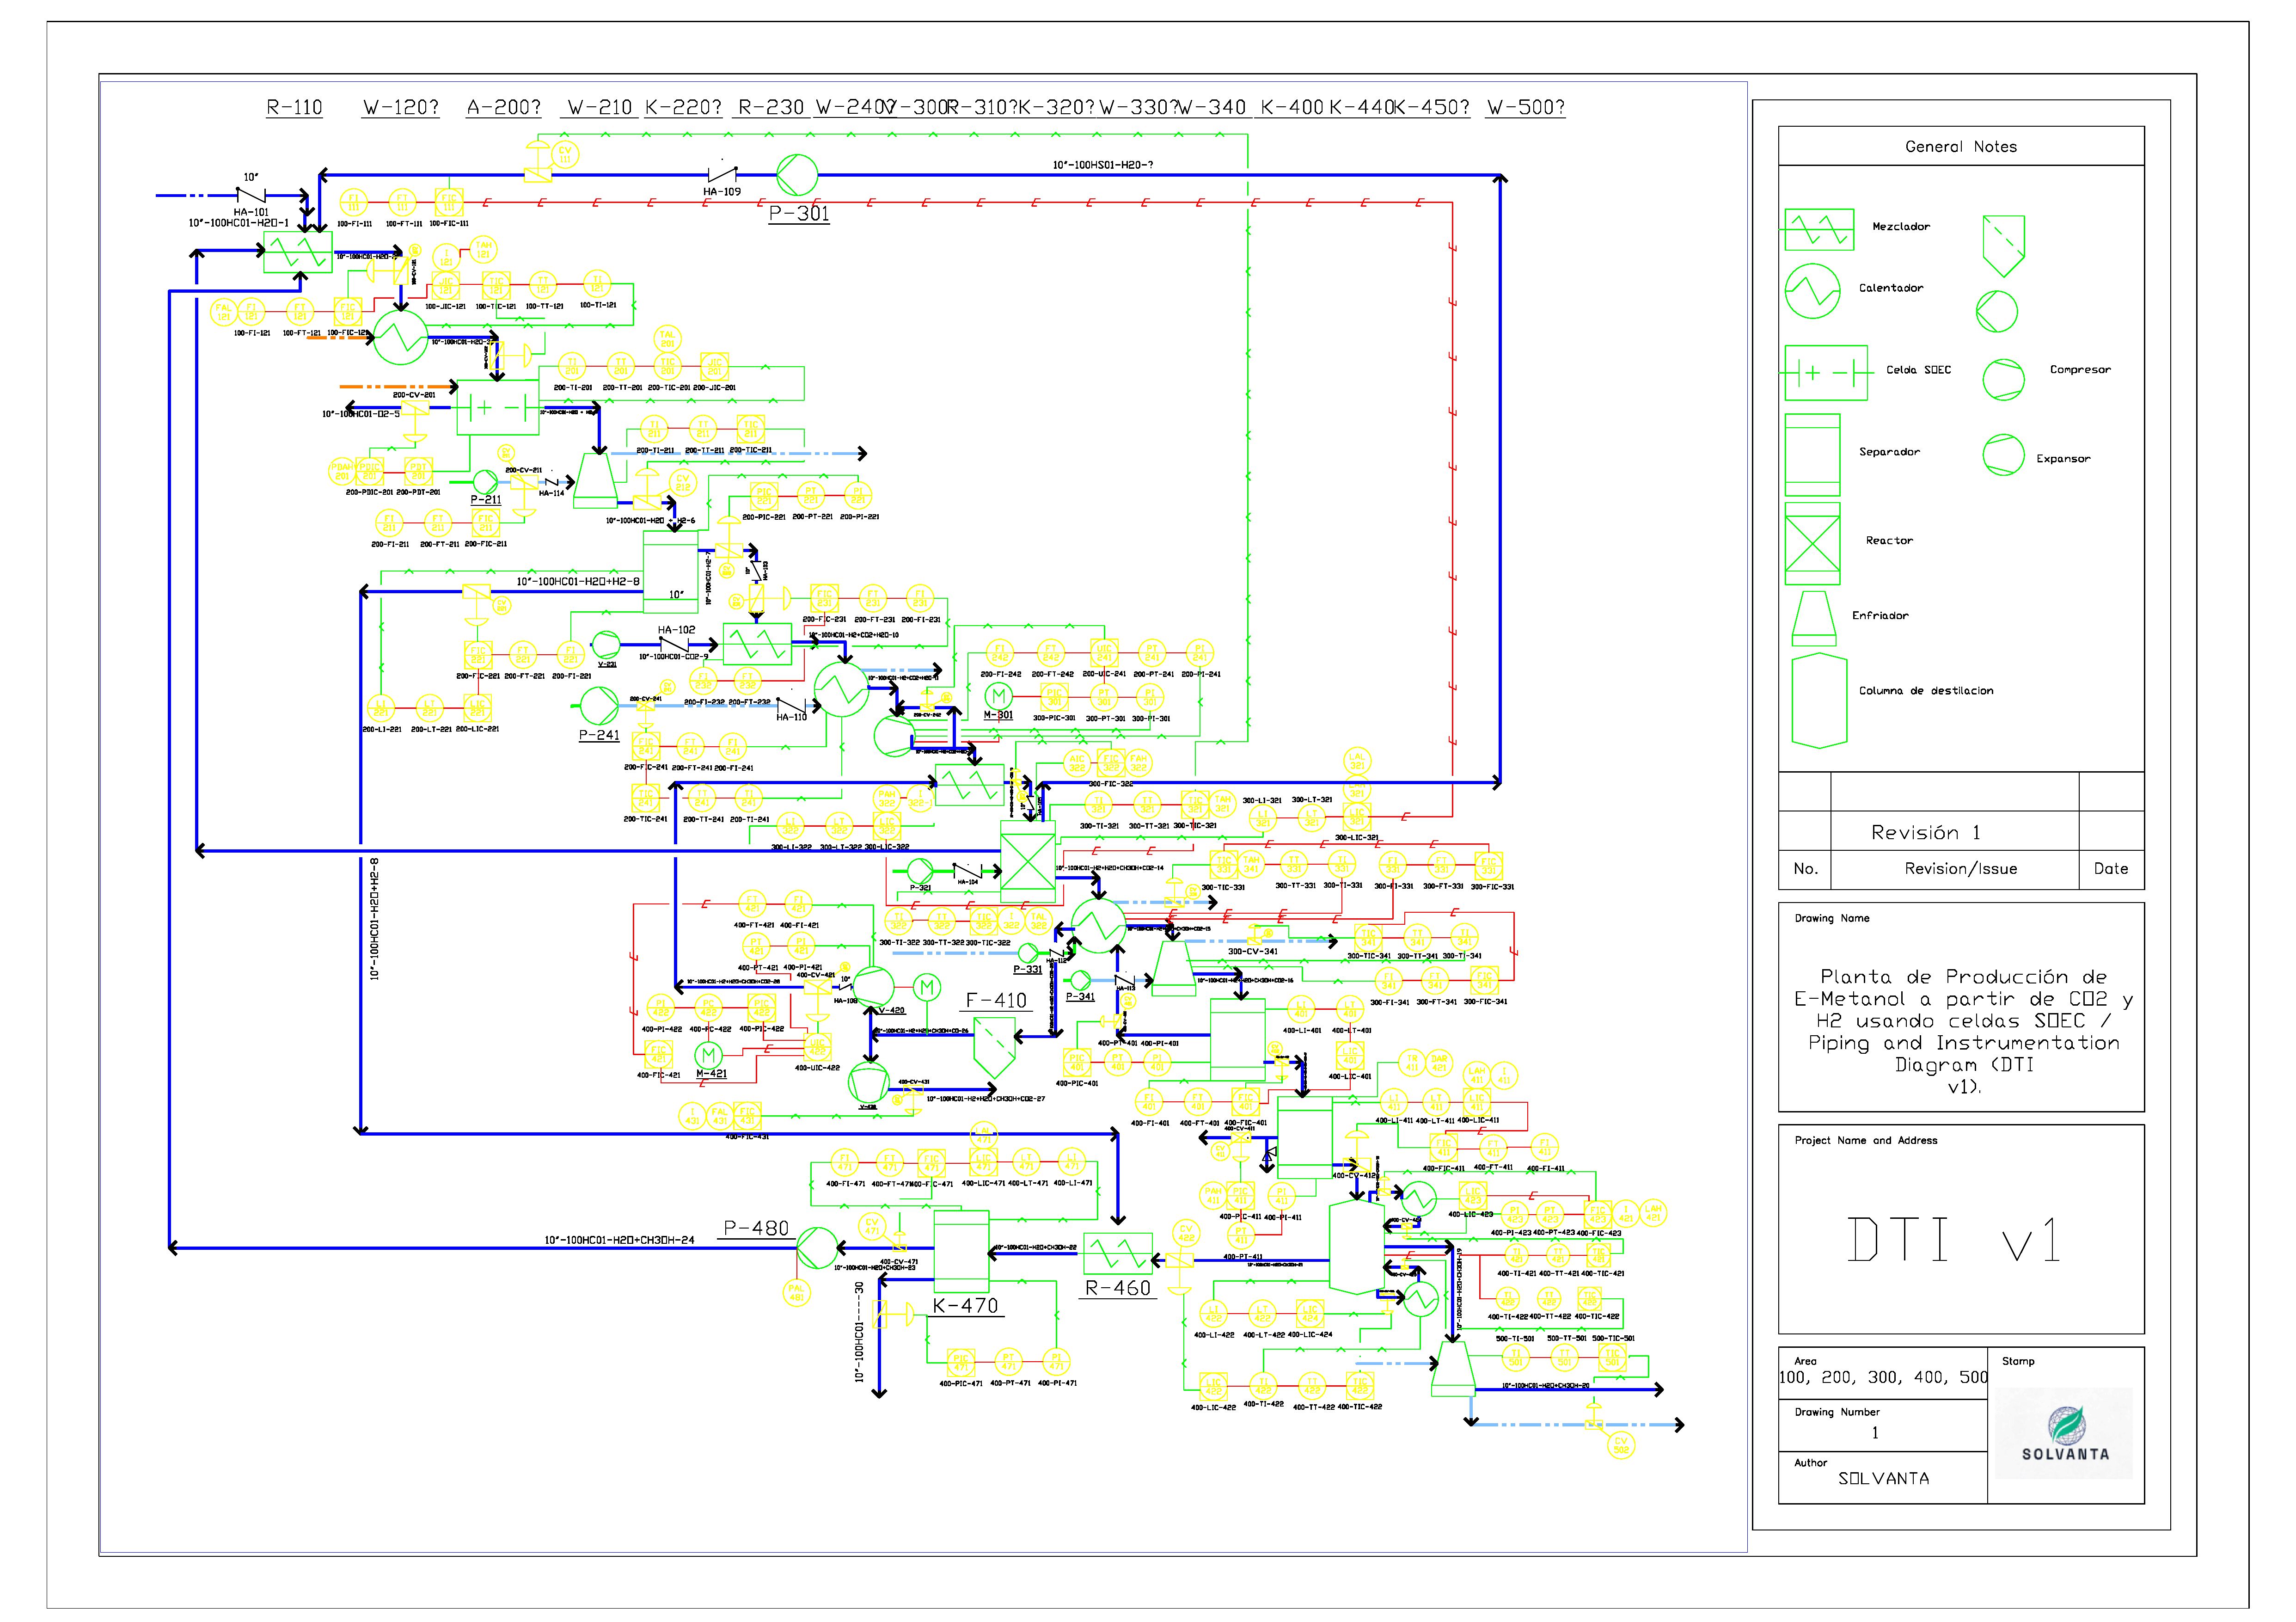
\includepdf[pages={1}, landscape=true, scale=0.92, pagecommand={\thispagestyle{fancy}}]{figuras/dti_v0_2.pdf}

\newpage
\subsection{Anexo D: Nomenclatura Oficial de Archivos Entregables}
La firma \textbf{Solvanta Engineering Solutions} generó y estructuró los ocho archivos oficiales conforme a las pautas de nomenclatura establecidas en la Sección 21 de la guía (Cuadro \ref{tab:nomenclatura_archivos}).

\begin{table}[H]
\centering\small
\setlength{\tabcolsep}{6pt}
\renewcommand{\arraystretch}{1.2}
\caption{\textbf{Nomenclatura oficial de archivos entregables del paquete PIB-01.}} \label{tab:nomenclatura_archivos}
\begin{tabularx}{\textwidth}{>{\bfseries}p{5.0cm} >{\ttfamily}p{6.0cm} X}
\toprule
\rowcolor{tableheader}
\color{white}\textbf{Documento de Entrega} & \color{white}\textbf{Nombre del Archivo Generado} & \color{white}\textbf{Descripción del Contenido Técnico} \\
\midrule
Expediente principal integrado & Solvanta\_PIB-01\_Expediente.pdf & Documento maestro en PDF con portada, memorias, formatos y anexos. \\ \addlinespace[2pt]
Bases consolidadas & Solvanta\_F-PIB-01.xlsx & Formato F-PIB-01 en Excel con 15 parámetros consolidados. \\ \addlinespace[2pt]
Inventario técnico de equipos & Solvanta\_F-PIB-02.xlsx & Formato F-PIB-02 en Excel con Partes A, B y C para los 30 equipos. \\ \addlinespace[2pt]
Balance de recursos y servicios & Solvanta\_F-PIB-03.xlsx & Formato F-PIB-03 en Excel con tasas y anualización de 24 conceptos. \\ \addlinespace[2pt]
Pendientes y verificación final & Solvanta\_F-PIB-04.xlsx & Formato F-PIB-04 en Excel con seguimiento de TBD, INC y HZ. \\ \addlinespace[2pt]
Arreglo general preliminar & Solvanta\_AG-01.pdf & Plano oficial de distribución en planta (Plot Plan) a escala. \\ \addlinespace[2pt]
DTI Versión 1 / Base analizada & Solvanta\_DTI\_v1.pdf & Plano DTI congelado de referencia con nodos y lazos SIS. \\ \addlinespace[2pt]
Tabla de corrientes de proceso & Solvanta\_TC-01.xlsx & Balance riguroso de las 36 corrientes en formato Excel. \\
\bottomrule
\end{tabularx}
\end{table}

\newpage
% ==============================================================================
% SECCIÓN 15: REFERENCIAS TÉCNICAS Y NORMATIVAS
% ==============================================================================
\section{Referencias Técnicas, Normativas y Bibliografía}

\begin{enumerate}[leftmargin=*]
    \item \textbf{Towler, G. y Sinnott, R.} (2021). \textit{Chemical Engineering Design: Principles, Practice and Economics of Plant and Process Design}. 6.ª edición. Butterworth-Heinemann / Elsevier.
    \item \textbf{Turton, R., Bailie, R. C., Whiting, W. B. y Shaeiwitz, J. A.} (2018). \textit{Analysis, Synthesis, and Design of Chemical Processes}. 5.ª edición. Prentice Hall / Pearson.
    \item \textbf{Green, D. W. y Southard, M. Z.} (2019). \textit{Perry’s Chemical Engineers’ Handbook}. 9.ª edición. McGraw-Hill Education.
    \item \textbf{Center for Chemical Process Safety (CCPS).} (2007). \textit{Guidelines for Safe Automation of Chemical Processes}. 2.ª edición. American Institute of Chemical Engineers (AIChE / CCPS). Wiley.
    \item \textbf{Center for Chemical Process Safety (CCPS).} (2008). \textit{Guidelines for Hazard Evaluation Procedures}. 3.ª edición. AIChE / CCPS. Wiley.
    \item \textbf{International Electrotechnical Commission (IEC).} (2016). \textit{IEC 61882: Hazard and Operability Studies (HAZOP Studies) -- Application Guide}. IEC, Ginebra, Suiza.
    \item \textbf{International Electrotechnical Commission (IEC).} (2016). \textit{IEC 61511: Functional Safety -- Safety Instrumented Systems for the Process Industry Sector}. Partes 1 a 3. IEC.
    \item \textbf{International Society of Automation (ISA).} (2009). \textit{ANSI/ISA-5.1-2009: Instrumentation Symbols and Identification}. ISA, Research Triangle Park, NC.
    \item \textbf{International Organization for Standardization (ISO).} (2000). \textit{ISO 10628: Flow Diagrams for Process Plants -- General Rules}. ISO, Ginebra, Suiza.
    \item \textbf{American Petroleum Institute (API).} (2012). \textit{API Recommended Practice 500: Recommended Practice for Classification of Locations for Electrical Installations at Petroleum Facilities}. 3.ª edición. API Publishing.
    \item \textbf{American Petroleum Institute (API).} (2014). \textit{API Standard 2000: Venting Atmospheric and Low-Pressure Storage Tanks}. 7.ª edición. API Publishing.
    \item \textbf{American Petroleum Institute (API).} (2020). \textit{API Standard 520: Sizing, Selection, and Installation of Pressure-Relieving Devices in Refineries}. Partes I y II. API Publishing.
    \item \textbf{American Society of Mechanical Engineers (ASME).} (2021). \textit{ASME Boiler and Pressure Vessel Code (BPVC), Section VIII: Rules for Construction of Pressure Vessels}. Divisiones 1 y 2. ASME, Nueva York.
    \item \textbf{Tubular Exchanger Manufacturers Association (TEMA).} (2019). \textit{Standards of the Tubular Exchanger Manufacturers Association}. 10.ª edición. TEMA Inc.
    \item \textbf{American Society for Testing and Materials (ASTM).} (2018). \textit{ASTM D1152-06(2018): Standard Specification for Methanol (Methyl Alcohol)}. ASTM International, West Conshohocken, PA.
    \item \textbf{DWSIM Chemical Process Simulator.} (2026). \textit{DWSIM Official Technical Documentation and Thermodynamics Reference Guide}. Versión 10.2.4.
    \item \textbf{Petróleos Mexicanos (PEMEX).} (2015). \textit{NRF-048-PEMEX-2015: Diseño de Instalaciones Eléctricas en Áreas Peligrosas}. Comité de Normalización de Pemex.
    \item \textbf{Petróleos Mexicanos (PEMEX).} (2017). \textit{NRF-036-PEMEX-2017: Clasificación de Áreas Peligrosas y Selección de Equipo Eléctrico}. Comité de Normalización de Pemex.
\end{enumerate}

\end{document}
